\documentclass[output=paper, colorlinks, citecolor=brown, booklanguage=german]{langscibook} 
\ChapterDOI{10.5281/zenodo.15471433}


\author{Ilse Zimmermann\affiliation{Zentrum für Allgemeine Sprachwissenschaft (ZAS), Berlin}}

% replace the above with you and your coauthors
% rules for affiliation: If there's an official English version, use that (find out on the official website of the university); if not, use the original
% orcid doesn't appear printed; it's metainformation used for later indexing

%%% uncomment the following line if you are a single author or all authors have the same affiliation
% \SetupAffiliations{mark style=none}

%% in case the running head with authors exceeds one line (which is the case in this example document), use one of the following methods to turn it into a single line; otherwise comment the line below out with % and ignore it
%\lehead{Šimík, Gehrke, Lenertová, Meyer, Szucsich \& Zaleska}
% \lehead{Radek Šimík et al.}
\title{Die Analysierbarkeit von Pronomen und Proadverbialia im Russischen}
% replace the above with your paper title
%%% provide a shorter version of your title in case it doesn't fit a single line in the running head
% in this form: \title[short title]{full title}
\abstract{\noabstract}

% % add all extra packages you need to load to this file

\usepackage{tabularx,multicol}
\usepackage{url}
\urlstyle{same}

\usepackage{listings}
\lstset{basicstyle=\ttfamily,tabsize=2,breaklines=true}

\usepackage{langsci-basic}
\usepackage{langsci-optional}
\usepackage{langsci-lgr}
\usepackage{langsci-osl}
% \usepackage{./langsci/styles/langsci-lgr}
% \usepackage{./langsci/styles/langsci-osl}
% \usepackage{langsci-gb4e}

\usepackage{tikz}
\usetikzlibrary{patterns,calc}
\pgfdeclarepatternformonly{south east lines}{\pgfqpoint{-0pt}{-0pt}}{\pgfqpoint{3pt}{3pt}}{\pgfqpoint{3pt}{3pt}}{
    \pgfsetlinewidth{0.6pt}
    \pgfpathmoveto{\pgfqpoint{0pt}{3pt}}
    \pgfpathlineto{\pgfqpoint{3pt}{0pt}}
    \pgfpathmoveto{\pgfqpoint{.2pt}{-.2pt}}
    \pgfpathlineto{\pgfqpoint{-.2pt}{.2pt}}
    \pgfpathmoveto{\pgfqpoint{3.2pt}{2.8pt}}
    \pgfpathlineto{\pgfqpoint{2.8pt}{3.2pt}}
    \pgfusepath{stroke}}
    
\usepackage{stmaryrd}
\usepackage{wasysym}
\usepackage{multirow}
\usepackage{caption}
\usepackage{subcaption}
\usepackage{mathrsfs}
\usepackage{qtree}

\usepackage{linguex}


% %pminos do not split footnotes
% \interfootnotelinepenalty=10000 %Footnote in Laporte chapters has to be split SN


%\DeclareIndexNameFormat{default}{%
%\nameparts{#1}%
%\usebibmacro{index:name}%
%{\index[names]}%
%{\namepartfamily}%
%{\namepartgiveni}%
% {}% L1
% {}% L2
%{\namepartprefix}% generates spurious space L3
%{\namepartsuffix}% generates spurious space L4
%}

%  {\DeclareIndexNameFormat{default}{%
%     \usebibmacro{index:name}{\index[names]}{#1}{#3}{#5}{#7}}}

%\DeclareIndexNameFormat{default}{%
%  \usebibmacro{index:name}{\sindex[nom]}{#1}{#3}{#5}{#7}}

%\DeclareIndexNameFormat{default}{%
%  \usebibmacro{index:name}{\sindex[person]}{#1}{#3}{#5}{#7}}
%\DeclareIndexNameFormat{default}{%
%\nameparts{#1} \usebibmacro{index:name}{\sindex[person]]}{\namepartfamily}{‌​\namepartgiven}{\nam‌​epartprefix}{\namepa‌​rtsuffix}}

%\newcommand{\smiley}{:)}

%\renewbibmacro*{index:name}[5]{%
%\usebibmacro{index:entry}{#1}%
%{\iffieldundef{usera}{}{\thefield{usera}\actualoperator}\mkbibindexname{#2}{#3}{#4}{#5}}}

% \newcommand{\noop}[1]{}

%remove for final
%\overfullrule=1mm

\newcommand{\tobi}[2]}}
\renewcommand{\S}[1]{\tobi{#1}{\textsc{*}}}

% this volume references
% puts: [this volume]
% already defined: \citetv
%\newcommand{\citepv}[1]{(\citeauthor{#1} \citeyear*{#1} [this volume])}
\newcommand{\citealtv}[1]{\citeauthor{#1} \citeyear*{#1} [this volume]}

%parentheses around example number
\newcommand{\pref}[1]{(\ref{#1})}

% in-text examples

\newcommand{\lnex}[1]{\textit{#1}} %target lang word
\newcommand{\lnlit}[1]{(lit.: `#1')} %literal reading
\newcommand{\lnlat}[1]{(#1)} % latinization
\newcommand{\lntrans}[1]{`#1'} %translation
\newcommand{\lnexl}[2]%
{\lnex{#1}{} \lnlat{#2}} % ex with latinization
\newcommand{\lnexlat}[3]{\lnex{#1}{} \lnlat{#2}{} \lntrans{#3}} % ex with latinization and tranl.

%ch01
\newcommand{\co}[1]{\mbox{\textbf{#1}}}

%ch09

\newcommand{\cyrbulg}[1]{\begin{otherlanguage*}{bulgarian}#1\end{otherlanguage*}}


%ch10
\newcommand{\nlp}{{\small NLP}}
\newcommand{\mwe}{{\small MWE}}
\newcommand{\rae}{{\small RAE}}
\newcommand{\lvc}{{\small LVC}}
\newcommand{\pos}{{\small P}o{\small S}}
%\newcommand{\todo}[1]{ \textcolor{red}{#1} }

%\renewcommand{\labelenumi}{\theenumi}
%\ainamefmt{{vv}{ll}{, ff}{, jj}} % fullname

\newcommand{\biberror}[1]{{\color{red}#1}}

\newcommand{\osenovaitem}{--~}
%
% \togglepaper[42]
% the chapter number will be provided by volume editors; for now keep this way

\begin{document}
\begin{otherlanguage}{german}
\maketitle

% Just comment out the input below when you're ready to go.
%For a start: Do not forget to give your Overleaf project (this paper) a recognizable name. This one could be called, for instance, Simik et al: OSL template. You can change the name of the project by hovering over the gray title at the top of this page and clicking on the pencil icon.

\section{Introduction}\label{sim:sec:intro}

Language Science Press is a project run for linguists, but also by linguists. You are part of that and we rely on your collaboration to get at the desired result. Publishing with LangSci Press might mean a bit more work for the author (and for the volume editor), esp. for the less experienced ones, but it also gives you much more control of the process and it is rewarding to see the quality result.

Please follow the instructions below closely, it will save the volume editors, the series editors, and you alike a lot of time.

\sloppy This stylesheet is a further specification of three more general sources: (i) the Leipzig glossing rules \citep{leipzig-glossing-rules}, (ii) the generic style rules for linguistics (\url{https://www.eva.mpg.de/fileadmin/content_files/staff/haspelmt/pdf/GenericStyleRules.pdf}), and (iii) the Language Science Press guidelines \citep{Nordhoff.Muller2021}.\footnote{Notice the way in-text numbered lists should be written -- using small Roman numbers enclosed in brackets.} It is advisable to go through these before you start writing. Most of the general rules are not repeated here.\footnote{Do not worry about the colors of references and links. They are there to make the editorial process easier and will disappear prior to official publication.}

Please spend some time reading through these and the more general instructions. Your 30 minutes on this is likely to save you and us hours of additional work. Do not hesitate to contact the editors if you have any questions.

\section{Illustrating OSL commands and conventions}\label{sim:sec:osl-comm}

Below I illustrate the use of a number of commands defined in langsci-osl.tex (see the styles folder).

\subsection{Typesetting semantics}\label{sim:sec:sem}

See below for some examples of how to typeset semantic formulas. The examples also show the use of the sib-command (= ``semantic interpretation brackets''). Notice also the the use of the dummy curly brackets in \REF{sim:ex:quant}. They ensure that the spacing around the equation symbol is correct. 

\ea \ea \sib{dog}$^g=\textsc{dog}=\lambda x[\textsc{dog}(x)]$\label{sim:ex:dog}
\ex \sib{Some dog bit every boy}${}=\exists x[\textsc{dog}(x)\wedge\forall y[\textsc{boy}(y)\rightarrow \textsc{bit}(x,y)]]$\label{sim:ex:quant}
\z\z

\noindent Use noindent after example environments (but not after floats like tables or figures).

And here's a macro for semantic type brackets: The expression \textit{dog} is of type $\stb{e,t}$. Don't forget to place the whole type formula into a math-environment. An example of a more complex type, such as the one of \textit{every}: $\stb{s,\stb{\stb{e,t},\stb{e,t}}}$. You can of course also use the type in a subscript: dog$_{\stb{e,t}}$

We distinguish between metalinguistic constants that are translations of object language, which are typeset using small caps, see \REF{sim:ex:dog}, and logical constants. See the contrast in \REF{sim:ex:speaker}, where \textsc{speaker} (= serif) in \REF{sim:ex:speaker-a} is the denotation of the word \textit{speaker}, and \cnst{speaker} (= sans-serif) in \REF{sim:ex:speaker-b} is the function that maps the context $c$ to the speaker in that context.\footnote{Notice that both types of small caps are automatically turned into text-style, even if used in a math-environment. This enables you to use math throughout.}$^,$\footnote{Notice also that the notation entails the ``direct translation'' system from natural language to metalanguage, as entertained e.g. in \citet{Heim.Kratzer1998}. Feel free to devise your own notation when relying on the ``indirect translation'' system (see, e.g., \citealt{Coppock.Champollion2022}).}

\ea\label{sim:ex:speaker}
\ea \sib{The speaker is drunk}$^{g,c}=\textsc{drunk}\big(\iota x\,\textsc{speaker}(x)\big)$\label{sim:ex:speaker-a}
\ex \sib{I am drunk}$^{g,c}=\textsc{drunk}\big(\cnst{speaker}(c)\big)$\label{sim:ex:speaker-b}
\z\z

\noindent Notice that with more complex formulas, you can use bigger brackets indicating scope, cf. $($ vs. $\big($, as used in \REF{sim:ex:speaker}. Also notice the use of backslash plus comma, which produces additional space in math-environment.

\subsection{Examples and the minsp command}

Try to keep examples simple. But if you need to pack more information into an example or include more alternatives, you can resort to various brackets or slashes. For that, you will find the minsp-command useful. It works as follows:

\ea\label{sim:ex:german-verbs}\gll Hans \minsp{\{} schläft / schlief / \minsp{*} schlafen\}.\\
Hans {} sleeps {} slept {} {} sleep.\textsc{inf}\\
\glt `Hans \{sleeps / slept\}.'
\z

\noindent If you use the command, glosses will be aligned with the corresponding object language elements correctly. Notice also that brackets etc. do not receive their own gloss. Simply use closed curly brackets as the placeholder.

The minsp-command is not needed for grammaticality judgments used for the whole sentence. For that, use the native langsci-gb4e method instead, as illustrated below:

\ea[*]{\gll Das sein ungrammatisch.\\
that be.\textsc{inf} ungrammatical\\
\glt Intended: `This is ungrammatical.'\hfill (German)\label{sim:ex:ungram}}
\z

\noindent Also notice that translations should never be ungrammatical. If the original is ungrammatical, provide the intended interpretation in idiomatic English.

If you want to indicate the language and/or the source of the example, place this on the right margin of the translation line. Schematic information about relevant linguistic properties of the examples should be placed on the line of the example, as indicated below.

\ea\label{sim:ex:bailyn}\gll \minsp{[} Ėtu knigu] čitaet Ivan \minsp{(} často).\\
{} this book.{\ACC} read.{\PRS.3\SG} Ivan.{\NOM} {} often\\\hfill O-V-S-Adv
\glt `Ivan reads this book (often).'\hfill (Russian; \citealt[4]{Bailyn2004})
\z

\noindent Finally, notice that you can use the gloss macros for typing grammatical glosses, defined in langsci-lgr.sty. Place curly brackets around them.

\subsection{Citation commands and macros}

You can make your life easier if you use the following citation commands and macros (see code):

\begin{itemize}
    \item \citealt{Bailyn2004}: no brackets
    \item \citet{Bailyn2004}: year in brackets
    \item \citep{Bailyn2004}: everything in brackets
    \item \citepossalt{Bailyn2004}: possessive
    \item \citeposst{Bailyn2004}: possessive with year in brackets
\end{itemize}

\section{Trees}\label{s:tree}

Use the forest package for trees and place trees in a figure environment. \figref{sim:fig:CP} shows a simple example.\footnote{See \citet{VandenWyngaerd2017} for a simple and useful quickstart guide for the forest package.} Notice that figure (and table) environments are so-called floating environments. {\LaTeX} determines the position of the figure/table on the page, so it can appear elsewhere than where it appears in the code. This is not a bug, it is a property. Also for this reason, do not refer to figures/tables by using phrases like ``the table below''. Always use tabref/figref. If your terminal nodes represent object language, then these should essentially correspond to glosses, not to the original. For this reason, we recommend including an explicit example which corresponds to the tree, in this particular case \REF{sim:ex:czech-for-tree}.

\ea\label{sim:ex:czech-for-tree}\gll Co se řidič snažil dělat?\\
what {\REFL} driver try.{\PTCP.\SG.\MASC} do.{\INF}\\
\glt `What did the driver try to do?'
\z

\begin{figure}[ht]
% the [ht] option means that you prefer the placement of the figure HERE (=h) and if HERE is not possible, you prefer the TOP (=t) of a page
% \centering
    \begin{forest}
    for tree={s sep=1cm, inner sep=0, l=0}
    [CP
        [DP
            [what, roof, name=what]
        ]
        [C$'$
            [C
                [\textsc{refl}]
            ]
            [TP
                [DP
                    [driver, roof]
                ]
                [T$'$
                    [T [{[past]}]]
                    [VP
                        [V
                            [tried]
                        ]
                        [VP, s sep=2.2cm
                            [V
                                [do.\textsc{inf}]
                            ]
                            [t\textsubscript{what}, name=trace-what]
                        ]
                    ]
                ]
            ]
        ]
    ]
    \draw[->,overlay] (trace-what) to[out=south west, in=south, looseness=1.1] (what);
    % the overlay option avoids making the bounding box of the tree too large
    % the looseness option defines the looseness of the arrow (default = 1)
    \end{forest}
    \vspace{3ex} % extra vspace is added here because the arrow goes too deep to the caption; avoid such manual tweaking as much as possible; here it's necessary
    \caption{Proposed syntactic representation of \REF{sim:ex:czech-for-tree}}
    \label{sim:fig:CP}
\end{figure}

Do not use noindent after figures or tables (as you do after examples). Cases like these (where the noindent ends up missing) will be handled by the editors prior to publication.

\section{Italics, boldface, small caps, underlining, quotes}

See \citet{Nordhoff.Muller2021} for that. In short:

\begin{itemize}
    \item No boldface anywhere.
    \item No underlining anywhere (unless for very specific and well-defined technical notation; consult with editors).
    \item Small caps used for (i) introducing terms that are important for the paper (small-cap the term just ones, at a place where it is characterized/defined); (ii) metalinguistic translations of object-language expressions in semantic formulas (see \sectref{sim:sec:sem}); (iii) selected technical notions.
    \item Italics for object-language within text; exceptionally for emphasis/contrast.
    \item Single quotes: for translations/interpretations
    \item Double quotes: scare quotes; quotations of chunks of text.
\end{itemize}

\section{Cross-referencing}

Label examples, sections, tables, figures, possibly footnotes (by using the label macro). The name of the label is up to you, but it is good practice to follow this template: article-code:reference-type:unique-label. E.g. sim:ex:german would be a proper name for a reference within this paper (sim = short for the author(s); ex = example reference; german = unique name of that example).

\section{Syntactic notation}

Syntactic categories (N, D, V, etc.) are written with initial capital letters. This also holds for categories named with multiple letters, e.g. Foc, Top, Num, etc. Stick to this convention also when coming up with ad hoc categories, e.g. Cl (for clitic or classifier).

An exception from this rule are ``little'' categories, which are written with italics: \textit{v}, \textit{n}, \textit{v}P, etc.

Bar-levels must be typeset with bars/primes, not with an apostrophe. An easy way to do that is to use mathmode for the bar: C$'$, Foc$'$, etc.

Specifiers should be written this way: SpecCP, Spec\textit{v}P.

Features should be surrounded by square brackets, e.g., [past]. If you use plus and minus, be sure that these actually are plus and minus, and not e.g. a hyphen. Mathmode can help with that: [$+$sg], [$-$sg], [$\pm$sg]. See \sectref{sim:sec:hyphens-etc} for related information.

\section{Footnotes}

Absolutely avoid long footnotes. A footnote should not be longer than, say, {20\%} of the page. If you feel like you need a long footnote, make an explicit digression in the main body of the text.

Footnotes should always be placed at the end of whole sentences. Formulate the footnote in such a way that this is possible. Footnotes should always go after punctuation marks, never before. Do not place footnotes after individual words. Do not place footnotes in examples, tables, etc. If you have an urge to do that, place the footnote to the text that explains the example, table, etc.

Footnotes should always be formulated as full, self-standing sentences.

\section{Tables}

For your tables use the table plus tabularx environments. The tabularx environment lets you (and requires you in fact) to specify the width of the table and defines the X column (left-alignment) and the Y column (right-alignment). All X/Y columns will have the same width and together they will fill out the width of the rest of the table -- counting out all non-X/Y columns.

Always include a meaningful caption. The caption is designed to appear on top of the table, no matter where you place it in the code. Do not try to tweak with this. Tables are delimited with lsptoprule at the top and lspbottomrule at the bottom. The header is delimited from the rest with midrule. Vertical lines in tables are banned. An example is provided in \tabref{sim:tab:frequencies}. See \citet{Nordhoff.Muller2021} for more information. If you are typesetting a very complex table or your table is too large to fit the page, do not hesitate to ask the editors for help.

\begin{table}
\caption{Frequencies of word classes}
\label{sim:tab:frequencies}
 \begin{tabularx}{.77\textwidth}{lYYYY} %.77 indicates that the table will take up 77% of the textwidth
  \lsptoprule
            & nouns & verbs  & adjectives & adverbs\\
  \midrule
  absolute  &   12  &    34  &    23      & 13\\
  relative  &   3.1 &   8.9  &    5.7     & 3.2\\
  \lspbottomrule
 \end{tabularx}
\end{table}

\section{Figures}

Figures must have a good quality. If you use pictorial figures, consult the editors early on to see if the quality and format of your figure is sufficient. If you use simple barplots, you can use the barplot environment (defined in langsci-osl.sty). See \figref{sim:fig:barplot} for an example. The barplot environment has 5 arguments: 1. x-axis desription, 2. y-axis description, 3. width (relative to textwidth), 4. x-tick descriptions, 5. x-ticks plus y-values.

\begin{figure}
    \centering
    \barplot{Type of meal}{Times selected}{0.6}{Bread,Soup,Pizza}%
    {
    (Bread,61)
    (Soup,12)
    (Pizza,8)
    }
    \caption{A barplot example}
    \label{sim:fig:barplot}
\end{figure}

The barplot environment builds on the tikzpicture plus axis environments of the pgfplots package. It can be customized in various ways. \figref{sim:fig:complex-barplot} shows a more complex example.

\begin{figure}
  \begin{tikzpicture}
    \begin{axis}[
	xlabel={Level of \textsc{uniq/max}},  
	ylabel={Proportion of $\textsf{subj}\prec\textsf{pred}$}, 
	axis lines*=left, 
        width  = .6\textwidth,
	height = 5cm,
    	nodes near coords, 
    % 	nodes near coords style={text=black},
    	every node near coord/.append style={font=\tiny},
        nodes near coords align={vertical},
	ymin=0,
	ymax=1,
	ytick distance=.2,
	xtick=data,
	ylabel near ticks,
	x tick label style={font=\sffamily},
	ybar=5pt,
	legend pos=outer north east,
	enlarge x limits=0.3,
	symbolic x coords={+u/m, \textminus u/m},
	]
	\addplot[fill=red!30,draw=none] coordinates {
	    (+u/m,0.91)
        (\textminus u/m,0.84)
	};
	\addplot[fill=red,draw=none] coordinates {
	    (+u/m,0.80)
        (\textminus u/m,0.87)
	};
	\legend{\textsf{sg}, \textsf{pl}}
    \end{axis} 
  \end{tikzpicture} 
    \caption{Results divided by \textsc{number}}
    \label{sim:fig:complex-barplot}
\end{figure}

\section{Hyphens, dashes, minuses, math/logical operators}\label{sim:sec:hyphens-etc}

Be careful to distinguish between hyphens (-), dashes (--), and the minus sign ($-$). For in-text appositions, use only en-dashes -- as done here -- with spaces around. Do not use em-dashes (---). Using mathmode is a reliable way of getting the minus sign.

All equations (and typically also semantic formulas, see \sectref{sim:sec:sem}) should be typeset using mathmode. Notice that mathmode not only gets the math signs ``right'', but also has a dedicated spacing. For that reason, never write things like p$<$0.05, p $<$ 0.05, or p$<0.05$, but rather $p<0.05$. In case you need a two-place math or logical operator (like $\wedge$) but for some reason do not have one of the arguments represented overtly, you can use a ``dummy'' argument (curly brackets) to simulate the presence of the other one. Notice the difference between $\wedge p$ and ${}\wedge p$.

In case you need to use normal text within mathmode, use the text command. Here is an example: $\text{frequency}=.8$. This way, you get the math spacing right.

\section{Abbreviations}

The final abbreviations section should include all glosses. It should not include other ad hoc abbreviations (those should be defined upon first use) and also not standard abbreviations like NP, VP, etc.


\section{Bibliography}

Place your bibliography into localbibliography.bib. Important: Only place there the entries which you actually cite! You can make use of our OSL bibliography, which we keep clean and tidy and update it after the publication of each new volume. Contact the editors of your volume if you do not have the bib file yet. If you find the entry you need, just copy-paste it in your localbibliography.bib. The bibliography also shows many good examples of what a good bibliographic entry should look like.

See \citet{Nordhoff.Muller2021} for general information on bibliography. Some important things to keep in mind:

\begin{itemize}
    \item Journals should be cited as they are officially called (notice the difference between and, \&, capitalization, etc.).
    \item Journal publications should always include the volume number, the issue number (field ``number''), and DOI or stable URL (see below on that).
    \item Papers in collections or proceedings must include the editors of the volume (field ``editor''), the place of publication (field ``address'') and publisher.
    \item The proceedings number is part of the title of the proceedings. Do not place it into the ``volume'' field. The ``volume'' field with book/proceedings publications is reserved for the volume of that single book (e.g. NELS 40 proceedings might have vol. 1 and vol. 2).
    \item Avoid citing manuscripts as much as possible. If you need to cite them, try to provide a stable URL.
    \item Avoid citing presentations or talks. If you absolutely must cite them, be careful not to refer the reader to them by using ``see...''. The reader can't see them.
    \item If you cite a manuscript, presentation, or some other hard-to-define source, use the either the ``misc'' or ``unpublished'' entry type. The former is appropriate if the text cited corresponds to a book (the title will be printed in italics); the latter is appropriate if the text cited corresponds to an article or presentation (the title will be printed normally). Within both entries, use the ``howpublished'' field for any relevant information (such as ``Manuscript, University of \dots''). And the ``url'' field for the URL.
\end{itemize}

We require the authors to provide DOIs or URLs wherever possible, though not without limitations. The following rules apply:

\begin{itemize}
    \item If the publication has a DOI, use that. Use the ``doi'' field and write just the DOI, not the whole URL.
    \item If the publication has no DOI, but it has a stable URL (as e.g. JSTOR, but possibly also lingbuzz), use that. Place it in the ``url'' field, using the full address (https: etc.).
    \item Never use DOI and URL at the same time.
    \item If the official publication has no official DOI or stable URL (related to the official publication), do not replace these with other links. Do not refer to published works with lingbuzz links, for instance, as these typically lead to the unpublished (preprint) version. (There are exceptions where lingbuzz or semanticsarchive are the official publication venue, in which case these can of course be used.) Never use URLs leading to personal websites.
    \item If a paper has no DOI/URL, but the book does, do not use the book URL. Just use nothing.
\end{itemize}
\vskip-2\baselineskip
\section{Aufgabenstellung}

Anhand des Russischen soll untersucht werden, inwieweit Pronomen und Proadverbialia morphosyntaktisch und semantisch analysierbar sind. Es ist zu klären, aus welchen lexikalischen und/oder funktionalen Einheiten sie gegebenenfalls bestehen und auf welchen Repräsentationsstufen welche wort- bzw. phrasenstrukturellen Konstituentenkonstellationen wirksam sind.

Ich beschränke mich auf \textit{k}-Wörter des Russischen in ihrer Beziehung zu ent\-sprechen\-den \textit{t}- (oder \textit{s'}-) und \textit{v}(\textit{e})\textit{s'}-Wörtern, die in charakteristischen Reihen bzw. in entsprechenden Proportionalgleichungen systematische Be\-deu\-tungs\-unter\-schiede signalisieren:\footnote{\label{fn:1}Das Adverb \textit{vsjako} `auf jede Weise' wird in den Wörterbüchern als vulgärsprachlich charakterisiert.}

%\ea\label{ex:02:ktv-reihe}
%\begin{tabularx}{\textwidth}{XXXX}
%    \textsc{person}      &   kto     & tot       & vse\\
%    \textsc{zeit}        & kogda     & togda     & vsegda\\
%    \textsc{ort}         & gde       & zdes'     & vezde\\
%    \textsc{richtung}    & kuda      & tuda      & \\
%    \textsc{art}         & kak       & tak       & vsjako\footnotemark\\
%                         & kakoj     & takoj     & vsjakij\\
%    \textsc{menge}       & skol'ko   & stol'ko   & \\
%    \end{tabularx}
%\z 

%\vspace{0,5cm}

\begin{table}[H]
\caption{Reihe von \textit{k}-Wörtern im Russischen}
\label{tab:reihen}
 \begin{tabularx}{.99\textwidth}{llll} %.77 indicates that the table will take up 77% of the textwidth
  \lsptoprule
\textsc{person} & \textit{kto} `wer' & \textit{tot} `jener' & \textit{vse} `alle'\\
\textsc{zeit} & \textit{kogda} `wann' & \textit{togda} `dann'&  \textit{vsegda} `immer'\\
\textsc{ort} & \textit{gde} `wo' & \textit{zdes'} `hier' & \textit{vezde} `überall'\\
\textsc{richtung} & \textit{kuda} `wohin' & \textit{tuda} `dorthin' & \\
\textsc{art} & \textit{kak} `wie' & \textit{tak} `so' & \textit{vsjako} `auf jede Weise'\\
& \textit{kakoj} `was für ein' & \textit{takoj} `ein solcher' & \textit{vsjakij} `jedweder'\\                
 \textsc{menge} & \textit{skol'ko} `wieviel' & \textit{stol'ko} `so viel' & \\
  \lspbottomrule
 \end{tabularx}
\end{table}

%\ea\label{ex:02:ktv-reihe}
%\ea \textsc{person}: \textit{kto} `wer', \textit{tot} `jener', \textit{vse} `alle'
%\ex \textsc{zeit}: \textit{kogda} `wann', \textit{togda} `dann', \textit{vsegda} `immer'
%\ex \textsc{ort}: \textit{gde} `wo', \textit{zdes'} `hier', \textit{vezde} `überall'
%\ex \textsc{richtung}: \textit{kuda} `wohin', \textit{tuda} `dorthin'
%\ex \textsc{art}: \textit{kak} `wie', \textit{tak} `so', \textit{vsjako} `auf jede Weise',
%\textti{kakoj} `was für einer', \textit{takoj} `ein solcher', \textit{vsjakij} `jedweder'                  
%\ex \textsc{menge}: \textit{skol'ko} `wieviel', \textit{stol'ko} `so viel'
%\z
%\z


\iffalse 

\ea\label{ex:02:ktv-reihe}
\begin{tabbing}
    \textsc{person}\hspace{1cm} \=  kto  \hspace{1cm}   \= tot  \hspace{1cm}    \=vse\\
    {}\hspace{2,1cm} \= ‘wer’ \> ‘jener’ \> ‘alle’ \\
    \textsc{zeit}               \>  kogda               \> togda                \> vsegda\\
    {}\hspace{2,1cm} \= ‘wann’ \> ‘dann’ \> ‘immer’ \\
    \textsc{ort}                \>  gde                 \> zdes'                \> vezde\\
    {}\hspace{2,1cm} \= ‘wo’ \> ‘hier’ \> ‘überall’ \\
    \textsc{richtung}           \>  kuda                \> tuda\\
    {}\hspace{2,1cm} \= ‘wohin’ \> ‘dorthin’  \\
    \textsc{art}                \>  kak                 \> tak                  \> vsjako\\
    {}\hspace{2,1cm} \= ‘wie’ \> ‘so’ \> ‘auf jede Weise’ \\
                                \>  kakoj               \> takoj                \> vsjakij\\
     {}\hspace{2,1cm} \= ‘…’ \> ‘…’ \> ‘jedweder’ \\                   
    \textsc{menge}              \>  skol'ko             \> stol'ko \\
    {}\hspace{2,1cm} \= ‘wie viel’ \> ‘so viel’  \\
\end{tabbing}
\z

\fi

\noindent \textit{k}-Wörter sind ihrerseits die Basis für Erweiterungen durch Partikeln, die Indefinita liefern, z.B.:

%\ea\label{ex:02:k-partikeln}
%    \begin{tabularx}{.5\textwidth}{XX}
%    koe-kto     & `jemand'\\
%    nikto       & `niemand'\\
%    kto-to      & `jemand'\\
%    kto-libo    & `irgendjemand'\\
%    kto-nibud'  & `irgendjemand'\\
%    \end{tabularx}
%\z

\ea\label{ex:02:k-partikeln}
%\begin{tabbing}
   \textit{koe-kto} `jemand' \\
   \textit{nikto} `niemand'\\
   \textit{kto-to} `jemand' \\
   \textit{kto-libo} `irgendjemand'\\
   \textit{kto-nibud'} `irgendjemand'\\
\z

\noindent Grammatiktheoretischer Rahmen ist das minimalistische Programm (\citealt{zi02:Chomsky1995,zi02:Chomsky1995,Chomsky1998,Chomsky1999}), erweitert um die Annahme, daß die Laut-Bedeutungs-Zu\-ord\-nung zwischen der Phonetischen Form (PF) und der Semantischen Form (SF) erfolgt (\citealt{Bierwisch1987,zi02:Bierwisch1997}). Die SF wird als Repräsentation der syste\-ma\-tischen, durch die Grammatik determinierten Bedeutung sprachlicher Ausdrücke angesehen und ist kompositional aus der Logischen Form (LF) abzuleiten. Bezüglich der Morphologie folge ich \citet{Stiebels.Wunderlich1994}, \citet{Wunderlich.Fabri1995} und \citet{Wunderlich1997a} in der Annahme, daß das Lexikon der Lieferant des wortstrukturellen Baumaterials ist. Allerdings gehört es zu den in dieser Untersuchung zu prüfenden Fragen, was es besagt, daß das Lexikon der Syntax als syntaktische Atome Wörter zur Verfügung stellt.

Ansatzpunkte für die Analyse sind u.a. Arbeiten von \citet{Katz.Postal1964}, \citet{Klima1964}, \citet{Postal1969}, \citet{Steinitz.Lang1969}, \citet{Zwarts1992}, \citet{Lenerz1993}, \citet{Cardinaletti1994}, \citet{Cardinaletti.Starke1995}, \citet{Rauh1995}, \citet{Acquaviva1995} und \citet{Tsai1999}, in denen die Analysierbarkeit von Pronomen und Proadverbialia essentiell zur Debatte steht.

In Abschnitt 2 stelle ich einige neuere Analysevorschläge vor, um bestimmte Gesichtspunkte deutlich zu machen, unter denen die Strukturierung von Pronomen und Proadverbialia untersucht wurde. Abschnitt 3 beinhaltet meine Analyse. Dabei wird weitere Literatur zur Sprache kommen. Abschnitt 4 ist ein kurzes Resümee.

\section{Einige Dekompositionsversuche für Pronomen und Proadverbialia} \label{dekompositionsversuche}

Je nach dem jeweiligen Schwerpunkt einzelner Untersuchungen und je nach der jeweiligen grammatiktheoretischen Auffassung haben Linguisten Pronomen und Proadverbialia als unanalysierte Ganzheiten betrachtet oder dekomponiert.\footnote{\citet{Nau1999} z.B. untersucht an europäischen und einigen australischen Sprachen den Formenbestand von Interrogativpronomen vom Typ \textit{wer, was} und \textit{welcher} bezüglich des Zusammenhangs von Kasusunterscheidungen und der semantisch-pragmatischen Kategorien Person, Bezugnahme auf eine im Kontext gegebene Menge von Entitäten und Spezifizität. Sie macht auf Lücken in den jeweiligen Paradigmen und Verwendungsweisen der Pronomen als \linebreak Interrogativ-, Indefinit- bzw. Relativpronomen aufmerksam. Eine morphosyntaktische Dekomposition und eine kategorielle Zuordnung der Ausdrücke werden nicht vorgenommen.} Mich interessieren Dekompositionsvorschläge, die vom Standpunkt der synchronischen Sprachbetrachtung gemacht wurden. \citet{Lenerz1993} setzt für Substantivgruppen eine morphosyntaktisch in funktionale und lexikalische Kategorien aufgegliederte Struktur an, deren Köpfe mit den ihnen zugewiesenen Formativen in (\ref{ex:02:formativa}) angedeutet sind.

%\ea\label{ex:02:formativa}
%    \begin{tabularx}{\textwidth}{llXXXX}
%    D   & DAgr  & AAgr  & A     & NAgr  & N\\
%    d   & en    & en    & schön & en    & Frau\\
%    d   & ich   &       &       &       & Idiot\\
%    w   & er    &       &       &       & e(mpty)\\
%        & er    &       &       &       & e(mpty)\\
%    \end{tabularx}
%\z 

\ea\label{ex:02:formativa}
\begin{tabbing}
    D   \hspace{1cm} \= DAgr \hspace{1cm}   \= AAgr  \hspace{1cm}  \= A \hspace{1cm}    \= NAgr \hspace{1cm}   \= N\\
    d                \> en                  \> en                   \> schön            \> en                   \> Frau\\
    d                \> ich                 \>                      \>                  \>                      \> Idiot\\
    w                \> er                  \>                      \>                  \>                      \> e(mpty)\\
                     \> er                  \>                      \>                  \>                      \> e(mpty)\\
\end{tabbing}
\z 

\noindent Die Flexive sind -- bis auf die von D -- den Stämmen immer übergeordnet und werden mit diesen per Kopfbewegung verknüpft. Für meine Fragestellung ist von Belang, daß Lenerz deutsche Pronomen wie \textit{mich} vs. \textit{dich} oder wie \textit{wer} vs. \textit{der} vs. \textit{er} durch Dekomposition systematisch zueinander ins Verhältnis setzt und auch die Erweiterbarkeit von Pronomen durch Modifikatoren wie in \textit{dich Idiot} berücksichtigt (vgl. auch \citealt{Zwarts1992}).

\citet{Cardinaletti1994} und \citet{Cardinaletti.Starke1995} nehmen für starke, schwache und klitische Personalpronomen eine unterschiedlich reiche interne morphosyntaktische Struktur an. Dabei bilden pronominale Klitika die am mei\-sten reduzier\-ten Ausdrücke, die nur aus D bestehen, das seinerseits morphologisch komplex sein kann (wie z.B. Italienisch \textit{lo} `ihn'/`es'), oder nur ein Flexiv darstellen (wie z.B. Deutsch \textit{m} für den Dativ Singular Maskulinum bzw. Neutrum; vgl. \textit{dem, ihm}). Starke Pronomen werden in NP erzeugt und in die DP oder noch höher in eine QP bewegt (wie z.B. Italienisch \textit{noi tutti} `wir alle'). Als Indiz für die Basisgenerierung starker Pronomen in NP sieht \citet{Cardinaletti1994} Mo\-di\-fi\-zier\-bar\-keit des Pronomens an (wie in Italienisch \textit{noi linguisti} `wir Linguisten', \textit{lui con i capelli rossi} `der mit den roten Haaren').

Es ist hier nicht der Platz, auf diese Strukturannahmen genauer einzugehen. Zu fragen ist, in welchem Maße sie sich in den hier zu betrachtenden Ausdrucksreihen des Russischen wiederfinden und wie sich die morphosyntaktische und die semantische Strukturierung der einzelnen Ausdrücke entsprechen, d.h. welche Bedeutungsanteile welchen wort- bzw. phrasenstrukturellen Einheiten zuzuordnen sind.

\citet{Acquaviva1995} untersucht Sätze mit mehrfacher Negation und schreibt Substantivgruppen mit quantifizierender Funktion eine Struktur wie in (\ref{ex:02:QDPN}) zu (vgl. auch \citealt{Giusti1991}).

\ea\label{ex:02:QDPN}
    [\textsubscript{QP} Q [\textsubscript{DP} D NP]]
\z 

\noindent Die Beispiele (\ref{ex:02:Kater}) und (\ref{ex:02:Wasser}) aus dem Italienischen (ebd., 79) zeigen, daß das Negativformativ durch den indefiniten Artikel mittels Kopfbewegung gestützt wird. Da Massenomen nicht mit overtem indefiniten Artikel auftreten, ist (\ref{ex:02:Wasser}) ungrammatisch.

\ea\label{ex:02:Kater}
    $[_\textrm{QP} [_\textrm{Q} [_\textrm{Q}\, \underset{\textrm{k}}{\textrm{ness}} ] [_\textrm{D}\, \underset{\textrm{ein}}{\textrm{un}} ]] [_\textrm{DP} \textrm{t} [_\textrm{NP}\, \underset{\textrm{Kater}}{\textrm{gatto}} ]]]$ \\
\z 

\begin{exe}
    \ex[*]{\label{ex:02:Wasser} $[_\textrm{QP} [_\textrm{Q} [_\textrm{Q}\, \underset{\textrm{k}}{\textrm{ness}} ] [_\textrm{D}\, \underset{\textrm{ein}}{\textrm{una}} ]] [_\textrm{DP}\, \textrm{t} [_\textrm{NP}\, \underset{\textrm{Wasser}}{\textrm{acqua}} ]]]$ \\
    }
\end{exe}

\noindent Die zentrale Annahme Acquavivas ist, daß mehrere FPs mit einer overten oder nichtoverten Negation in einer Konstruktion ein komplexes Interpretationsobjekt bilden derart, daß nur die hierarchisch höchste Negation semantisch wirksam wird. Wir werden auf entsprechende Konstruktionen des Russischen zurückkommen.

\citet{Tsai1999} macht am Chinesischen deutlich, daß die Pendants zu deutschen w-Wörtern wie z.B. \textit{shenme} `was' als Indefinit- bzw. als Interrogativpronomen fungieren können und die Basis für Zusätze mit Binderfunktion bilden wie in \textit{shenme-dou} `alles'. Tsai plädiert überzeugend dafür, die elementaren w-Wörter semantisch mit einer ungebundenen Variablen zu repräsentieren und diese in Abhängigkeit vom Satztyp bzw. von der Zugehörigkeit der betreffenden Phrase zum restrictive clause bzw. zum nuclear scope in der jeweiligen Konstruktion Bindungsoperationen zu unterziehen.\footnote{Zur Aufteilung von Sätzen in die beiden Interpretationsbereiche restrictive clause und nuclear scope und zur Unterscheidung spezifischer und unspezifischer Indefinita siehe \citet{Heim1982} und \citet{Diesing1992}.} 

\citet[10f., 31ff.]{Tsai1999} sieht auch wesentliche Zusammenhänge zwischen der Position der Binder und bestimmten Beschränkungen für Konstituentenbewegungen in verschiedenen Sprachen. So können die w-Insel-Beschränkung und die Komplexe-NP-Beschränkung (s. \citealt{Ross1967}) im Chinesischen im Unterschied zum Englischen nicht verletzt werden. Im Chinesischen bleibt die w-Phrase in situ und an der Satzspitze figuriert in Interrogativsätzen ein phonologisch leerer O\-pe\-ra\-tor. Im Englischen dagegen wird das w-Wort in N mit dem Ope\-ra\-tor verknüpft und in die satzinitiale Position bewegt, wobei es zu den genannten Verletzungen kommen kann. Vgl. folgende Strukturen:

\ea\label{ex:02:shenme}
    $[_\textrm{CP}\, \textrm{Op}_\textrm{Q}\, [_\textrm{IP}\, \dots \textrm{shenme} \dots ]]$
\z 

\ea\label{ex:02:what}
    $[_\textrm{CP} [_\textrm{IP}\, \dots [_\textrm{N}\, [_\textrm{N}\, \textrm{what} ]\, \textrm{Op}_\textrm{Q} ] \dots ]] \rightarrow \newline [_\textrm{CP}\, [_\textrm{N}\, [_\textrm{N}\, \textrm{what} ] \textrm{Op}_\textrm{Q} ]_\textrm{i}\, [_\textrm{IP}\, \dots \textrm{t}_\textrm{i} \dots ]]$
\z 

\noindent Es soll hier nicht diskutiert werden, inwieweit die Einzelheiten der vorgeschlagenen Analyse tragfähig sind.\footnote{Mir erscheint die fürs Englische angenommene Analyse der wh-Pronomen nicht zwingend. Mindestens der wh-Teil von \textit{what} könnte analog zu dem th-Teil von \textit{that} in D platziert sein, so daß NP als entscheidender Grenzknoten für Bewegung nicht ins Gewicht fallen könnte. Ohnehin bewegt sich nicht N, wo Tsai \textit{wh+at+}Op\textsubscript{Q} platziert, sondern die ganze DP oder eine noch umfassendere Phrase, wie z.B. \textit{for what}.} Wichtig wird sein, die entsprechenden pro\-no\-mi\-na\-len Ausdrücke des Russischen hinsichtlich der Aufgliederung in einen Ope\-ra\-tor\-teil und weitere Komponenten und die Zuordnung der Teile zu morpho\-syntaktischen Kategorien genau zu beleuchten.

Im folgenden Abschnitt präsentiere ich meine Vorschläge, morphosyntaktisch und semantisch relativ durchsichtig strukturierte Pronomen und Proadverbialia zu dekomponieren. Dabei gehe ich davon aus, daß die zu untersuchenden Einheiten DPs bzw. PPs mit der in Abbildung \ref{fig:internestruktur} gezeigten internen Struktur sind. 

\begin{figure} 
    \centering
    \begin{forest}
    for tree={parent anchor=south, child anchor=north}
        [(PP) 
            [(P) [$\varnothing$, tier=bottom] ]
            [DP 
                [D  
                    [(Partikel) [koe/ni, tier=bottom] ] 
                    [D, calign=first [D [D [k/t/v(e)s', tier=bottom] ]] [(Flexiv)]] 
                    [(Partikel) [to/nibud'/\dots, tier=bottom] ]]
                [NP 
                    [NP [N [$\varnothing$/de/gda/k/da/du, tier=bottom]]] 
                    [(AP/PP/CP)]] 
            ]
        ]
    \end{forest}
    \caption{Morphosyntaktische Struktur der untersuchten russischen Pronomina und Proadverbialia}
    \label{fig:internestruktur}
\end{figure}

Die Analyse verfolgt größte Einheitlichkeit der Dekomposition von Pronomen und Proadverbialia mit der Strukturierung von PPs und DPs (s. \citealt{Steube.Spaeth1998,Zimmermann1999}). Ich betrachte Pronomen wie \textit{kto} `wer' als DP, Proadverbialia wie \textit{kogda} `wann' als PP und beziehe wie \citet{Lenerz1993} und \citet{Cardinaletti1994} restringierende Modifikatoren, APs, PPs oder CPs, in die Analyse ein. Es sei von Anfang an klar, daß ich hier Pronomen und Proadverbialia ausschließlich unter synchronischem Gesichtspunkt beleuchte.

\section{Die Dekomposition der russischen \textit{k}-Wörter und ihrer Derivate} \label{analyse}

Bei den Pronomen und Proadverbialia sind folgende syntaktische Klassen zu unterscheiden: Ds wie \textit{tot} `der'/`jener', DPs wie \textit{kto} `wer', APs wie \textit{kakoj} `was für ein' und PPs wie \textit{gde} `wo'. Semantisch handelt es sich um Operatoren, Terme und Prädikate. Dabei wird zu klären sein, welche Zuordnungen der morpho\-syn\-takti\-schen Komponenten zu bestimmten Bedeutungsanteilen der Ausdrücke bestehen. Im Vordergrund des Interesses steht die Reihenbildung, und zwar die Gegenüberstellung der \textit{t}-Reihe und der \textit{k}-Reihe und ein Seitenblick auf die \textit{v(e)s'}-Reihe. Wir haben zu fragen, was die Varianz und die Invarianz dieser Reihen ausmacht und wie sich die oben genannten syntaktischen und semantischen Klassifizierungen und Funktionen ergeben. Den Schwerpunkt der Betrachtung bilden die \textit{k}-Wörter in ihrer Mehrfunktionalität als Interrogativ- und Relativpronomen und -adverbialia und als Basis für die Bildung von indefiniten Pronomen und Adverbialia mittels Erweiterung durch Partikeln.\footnote{Unter die Mehrfunktionalität der \textit{k}-Wörter fällt auch ihre Verwendung an der Spitze von Ex\-kla\-mativ\-sätzen, wie \citet[157]{Peskovskij1956} vermerkt. Ich lasse diese Konstruktionen beiseite (s. dazu \citealt{Zybatow1990}).} Es werden adverbielle und substantivische Prowörter behandelt. Adjektivische Prowörter lasse ich beiseite.

Ich unterscheide bei der morphosyntaktischen Analyse der Ausdrücke zwei Strukturebenen:

\ea\label{ex:02:strukturebenen}
    \ea\label{ex:02:strukturebenen-a} $([_\textrm{PP}\, \textrm{P})_{\alpha}\, [_\textrm{DP}\, [_\textrm{D}\, \textrm{(Partikel)}_{\beta}\, [_\textrm{D}\, [_\textrm{D}\, \textrm{Determinator} ] \newline \textrm{Flexiv} ]\, \textrm{(Partikel)}_{-\beta} ] [_\textrm{NP}\, [_\textrm{N}\, \textrm{Stützmorphem} ]]](])_{\alpha}$
    
    \ex\label{ex:02:strukturebenen-b} $([_\textrm{PP}\, \textrm{P})_{\alpha}\, [_\textrm{DP}\, [_\textrm{D}\, \textrm{(Partikel)}_{\beta}\, [_\textrm{D}\, [_\textrm{D}\, [_\textrm{D}\, \textrm{Determinator} ] \newline \textrm{Flexiv} ] [_\textrm{N}\, \textrm{Stützmorphem} ]]\, \textrm{(Partikel)}_{-\beta} ]](])_{\alpha}$
\z\z 

\noindent (\ref{ex:02:strukturebenen-a}) repräsentiert die für die Ebene der LF geltende syntaktische Strukturierung. (\ref{ex:02:strukturebenen-b}) zeigt die Eingabe in die PF, nämlich die Adjunktion des (gegebenenfalls phonologisch leeren) Stützmorphems in N an den möglicherweise flektierten Determinator. (\ref{ex:02:niemand})--(\ref{ex:02:uberall}) sind Beispiele für diese abgeleitete Struktur.\footnote{In den morphosyntaktischen Repräsentationen und den Lexikoneinträgen verzichte ich auf eine phonologische Charakterisierung der Formative.}

\ea\label{ex:02:niemand} $[_\textrm{DP}\, [_\textrm{D}\, \textrm{ni}\, [_\textrm{D}\, [_\textrm{D}\, [_\textrm{D}\, \textrm{k} ]\, \textrm{ogo} ] [_\textrm{N}\, \varnothing ]]]]$
\jambox*{`niemanden'}
\z 

\ea\label{ex:02:damals} $[_\textrm{PP}\, [_\textrm{P}\, \varnothing ] [_\textrm{DP}\, [_\textrm{D}\, [_\textrm{D}\, [_\textrm{D}\, \textrm{t}\, ]\, \textrm{o}\, ] [_\textrm{N}\, \textrm{gda} ]]]]$
\jambox*{`damals'}
\z 

\ea\label{ex:02:uberall} $[_\textrm{PP}\, [_\textrm{P}\, \varnothing ] [_\textrm{DP}\, [_\textrm{D}\, [_\textrm{D}\, \textrm{ves'}\, ] [_\textrm{N}\, \textrm{de} ]]]]$ (=\textit{vezde})
\jambox*{`überall'}
\z 

\noindent Restringierende, in Abbildung \ref{fig:internestruktur} vorgesehene Modifikatoren zu Pronomen und Proadverbialia wie in \textit{kto iz vas} `wer von euch', \textit{koe-čto interesnoe} `etwas Interessantes' oder \textit{gde-nibud' v Moskve} `irgendwo in Moskau' haben NP zum Modifikandum. Deshalb sind Stützmorpheme der Proausdrücke in LF unter NP und erst in PF unter D repräsentiert.

Für die Semantik der DPs setze ich folgende Komponenten voraus (siehe \citealt{Zimmermann1999}):

\ea\label{ex:02:komponenten}
    \gll {Op $x$} {[$ \dots x \dots ]$} {$[ \dots x \dots ]$}\\
    Operator {restrictive clause} {nuclear scope}\\
\z 

\noindent Ich gehe davon aus, daß diese Dreiteilung durch die Semantik der Determinatoren bereitgestellt wird.

Die Einzelheiten dieser Annahmen werden in den folgenden Abschnitten ver\-deut\-licht werden. Im Abschnitt \ref{sec:zi02:relativ} werden Relativsätze betrachtet, im Abschnitt \ref{sec:zi02:interrogativ} Interrogativsätze und im Abschnitt \ref{sec:zi02:indefinit} Indefinitpronomen, deren Basis \textit{k}-Wörter sind. Abschnitt \ref{sec:zi02:allquant} ist ein kurzer Exkurs in den Bereich von allquantifizierten Ausdrücken. Abschnitt \ref{sec:zi02:reichweite} hinterfragt die Reichweite der vorgeschlagenen Analyse. Abschnitt \ref{sec:zi02:alternative} stellt einen alternativen Analyseansatz zur Diskussion. 

\subsection{\textit{k}-Wörter in Relativsätzen}\label{sec:zi02:relativ}

\textit{k}-Pronomen und -adverbialia treten an der Spitze von Relativsätzen auf, und zwar von solchen mit einer Bezugsphrase in der übergeordneten Konstruktion als auch in freien Relativsätzen, ohne eine explizite Bezugsphrase.\footnote{Das Beispiel (\ref{ex:02:fenster}) ist \citet[108]{Mamonov.Rozental1957} entnommen, wo auch die Kongruenz\-re\-gu\-laritäten in solchen Konstruktionen behandelt werden.}

\ea\label{ex:02:fenster}
    \gll Te, kto ne uspel(i) k dveri, kinulis' k oknam.\\
    die wer \textsc{neg} schaffte zur Tür stürzten zu Fenstern\\
    \glt ‘Die, die es nicht zur Tür geschafft hatten, stürzten zu den Fenstern.’
\z 

\ea\label{ex:02:fenster-2}
    \gll Kto ne uspel k dveri, kinulsja k oknam.\\
    wer nicht schaffte zur Tür stürzte zu Fenstern\\
    \glt ‘Wer es nicht zur Tür geschafft hatte, stürzte zu den Fenstern.’
\z 

\ea\label{ex:02:dom}
    \gll Dom, gde ja rodilas', ustranili.\\
    Haus wo ich geboren beseitigten\\
    \glt ‘Das Haus, in dem ich geboren wurde, gibt es nicht mehr (wörtlich: haben sie beseitigt).’
\z 

\noindent Genau wie in Interrogativsätzen befindet sich im Russischen auch in Relativsätzen die Phrase mit dem \textit{k}-Wort an der linken Satzperipherie, in SpecCP. Das \textit{k}-Wort legitimiert dort seine Kategorisierung als $+$rel-Einheit, und zwar in Spe\-zi\-fi\-ka\-tor-Kopf-Konfiguration mit C, das auch dieses Merkmal hat. Für die semantische Interpretation solcher Relativsätze nehme ich an, daß auf der Ebene der LF die an die Satzspitze bewegte Phrase getilgt wird und die Kopie in situ semantisch wirksam wird, und zwar zusammen mit der SF von C mit der Kenn\-zeichnung $+$rel. (\ref{ex:02:lexikoneintrag-c}) skizziert den Lexikoneintrag für dieses C.\footnote{Zu den Informationstypen von Lexikoneinträgen siehe \citet{Jackendoff1975}.}

\newpage
\ea\label{ex:02:lexikoneintrag-c}
    \ea /\varnothing/
    \ex $+$C $+$rel
    \ex $\lambda Q\, \lambda X\, \exists s\, [Q\, s]$ mit\, $Q \in \langle e,t\rangle, X \in \{e, t,\, \langle e,t\rangle \}$
    \z
\z 

\noindent Demnach ist dieses C phonologisch leer, syntaktisch als $+$C $+$rel kategorisiert und semantisch der Binder des referentiellen Arguments des Verbs und zugleich Lieferant einer Argumentstelle, $\lambda X$. Dabei ist vorausgesetzt, daß $Q$ mindestens ein Vorkommen einer entsprechenden freien Variablen $X$ enthält. 

Das muß das Relativpronomen in situ garantieren. Es hat ja -- nach meinen Annahmen über die Dekomposition der \textit{k}-Wörter -- mindestens einen Operatorteil, einen Restriktorteil und einen weiteren Teil für den nuclear scope. Der Operatorteil blockiert $\lambda X$ als Argumentstelle und macht die entsprechenden Variablen im Restriktor und im nuclear scope dadurch greifbar für den Operator in C. (\ref{ex:02:lexikoneintrag-d}) ist der Lexikoneintrag für D von \textit{k}-Wörtern in der Funktion als Relativ- bzw. Interrogativpronomen und -ad\-verbia\-lia.

\ea\label{ex:02:lexikoneintrag-d}
    \ea\label{ex:02:lexikoneintrag-d-a} /k/
    \ex\label{ex:02:lexikoneintrag-d-b} $+$D $+$w $+$rel resp. $+$interr $\alpha$max
    \ex\label{ex:02:lexikoneintrag-d-c} $[_\textrm{D}\, [_\textrm{D} \_\_ \textrm{(X)} ]\, \textrm{N} ]$
    \ex\label{ex:02:lexikoneintrag-d-d} $\lambda P\, \lambda Q\, [ P\, x ][ Q\, x ]$ mit $P, Q \in \langle e, t\rangle$
    \z
\z

\noindent Ich nehme an, daß die morphosyntaktische Klassifizierung der \textit{k}-Wörter als Re\-la\-tiv- bzw. Interrogativpronomen oder -adverbial von D ausgeht. Das trifft auch für die Klassifizierung der Indefinita zu, die auf der Basis von \textit{k}-Wörtern gebildet sind. Alle diese Wörter haben das Merkmal $+$w, was für die Morphemselektion relevant ist. $\alpha$max in (\ref{ex:02:lexikoneintrag-d-b}) ist ein wortstrukturelles Merkmal, das das Formativ \textit{k} als Stamm bzw. als syntaktisches Atom charakterisiert. In (\ref{ex:02:lexikoneintrag-d-c}) ist \textit{k} (mit einer möglichen flexivischen Erweiterung) als gebundenes Morphem ausgewiesen. Es bedarf in  PF der Stützung durch ein N.

Durch die dem Formativ \textit{k} bei Relativ- und Interrogativpronomen und -ad\-verbialia zugeordnete semantische Operation entsteht nach Amalgamierung mit der SF der NP ein Term vom Typ $\langle\langle e, t\rangle, t\rangle$, mit dem Restriktor, der den Wer\-te\-be\-reich charakterisiert (Person, Ort, Zeit etc.), und dem zu spezifizierenden nuclear scope. In beiden Teilen figuriert $x$ als freie Variable, bewirkt durch die \textit{k} in (\ref{ex:02:lexikoneintrag-d-a}) zugeordnete Semantik.

Das Relativpronomen \textit{kto} in (\ref{ex:02:fenster}) und (\ref{ex:02:fenster-2}) hat dann folgende morpho\-syn\-tak\-ti\-sche LF-Struktur und SF:

\newpage
\ea
    \ea\label{ex:02:kto-lf} $[_\textrm{DP}\, [_\textrm{D}\, [_\textrm{D}\, \textrm{k} ]\, \textrm{to} ] [_\textrm{NP}\, [_\textrm{N}\, \varnothing ]]]$
    \ex\label{ex:02:kto-sf} $\lambda Q\, [\cnst{PERSON}\, x] [ Q\, x ]$
    \z
\z 

\noindent Das relativische Adverbial \textit{gde} in (\ref{ex:02:dom}) ist auf diesen beiden Repräsentationsebenen folgendermaßen strukturiert:

\ea
    \ea\label{ex:02:gde-lf} $[_\textrm{PP}\, [_\textrm{P}\, \varnothing ][_\textrm{DP}\, [_\textrm{D}\, \textrm{k} ] [_\textrm{NP}\, [_\textrm{N}\, \textrm{de} ]]]]$
    \ex\label{ex:02:gde-sf} $\lambda y\, [\cnst{ORT}\, \textrm{x} ] [ y\, R\, x ]$
\z\z 

\noindent In (\ref{ex:02:kto-lf}) ist \textit{to} als semantisch leeres Formativ \textit{k} angefügt, während $\varnothing\,$ in NP als Lieferant des Prädikats $\lambda x [\textsc{person}\, x ]$ zur Charakterisierung des Restriktors \mbox{dient}.\footnote{Nur der Nominativ von \textit{kto} und der Nominativ und Akkusativ von \textit{čto} weisen das hier semantisch leere Formativ \textit{to} auf. Alle anderen Formen dieser beiden Pronomen bestehen aus dem Operatormorphem und Kasusendungen. Zur Charakterisierung des Restriktors nehme ich ein phonologisch leeres N an.} In (\ref{ex:02:gde-lf}) liefert das Formativ \textit{de} in NP das Prädikat $\lambda x\, [\textsc{ort}\, x ]$, ebenfalls zur Charakterisierung des Restriktors. Die phonologisch leere Präposition bewirkt die Adverbialisierung für \textit{gde} und bringt eine unspezifische Relation zu einem neuen Argument $y$ ein, das als Anknüpfungspunkt an einen Modifikanden \mbox{dient}.\footnote{\label{fn:10} Die SF (\ref{ex:02:gde-sf}) resultiert aus der Amalgamierung folgender Bedeutungsbestandteile (genauer dazu s. Abschnitt \ref{sec:zi02:indefinit-2}.):
    \ea $\lambda$\textfrak{R} $\lambda y\, [$\textfrak{R} $\lambda x\, [ y\, R\, x ]] (\lambda P\, \lambda Q\, [P x] \, [ Q x\, ] (\lambda x\, [\cnst{ORT}\, x]))$
    \z 
} Wenn man annimmt, daß Bedeutung tragende Präpositionen das Merkmal $+$adv haben und wenn man die für Proadverbiale typischen Formative wie \textit{de} (für Ort), \textit{gda} (für Zeit) ebenfalls mit dem Merkmal $+$adv kennzeichnet, könnte für die in (\ref{ex:02:gde-lf}) angenommene Konstellation von Konstituenten \citeauthor{zi02:Emonds1987}' (\citeyear{zi02:Emonds1987}) E(mpty) H(ead) P(rinciple) geltend gemacht weren, nach dem eine leere Kategorie legitimiert ist, wenn sie in der Schwesterkonstituente ausgedrückt ist.

Das ist alles, was zu solchen als Relativsatzeinleitung fungierenden \textit{k}-Wörtern zu sagen ist. Die vorgeschlagene Behandlung ist denkbar einfach und kor\-res\-pon\-diert gut mit Gegebenheiten in anderen Sprachen, die die \textit{w}-Wörter auch syntaktisch in situ belassen (s. \citealt{Tsai1999}), und mit den folgenden für Interrogativsätze zu machenden Annahmen.

\subsection{\textit{k}-Wörter in Interrogativsätzen}\label{sec:zi02:interrogativ}

Für Interrogativsätze mit dem Interrogativpronomen oder -adverbial in SpecCP nehme ich -- ganz analog zu der Behandlung der Relativsätze -- an, daß die Bewegung der Phrase mit dem \textit{k}-Wort an die linke Satzperipherie in LF durch Tilgung rückgängig gemacht wird und die semantische Interpretation der Phrase in situ erfolgt, wieder im Zusammenwirken mit einem durch C eingeführten Operator. Der Lexikoneintrag für das interrogativische C sieht so aus:

\ea\label{ex:02:lexikoneintrag-c-interr}
    \ea /\varnothing/
    \ex\label{ex:02:lexikoneintrag-c-interr-b} $+$C $+$interr
    \ex\label{ex:02:lexikoneintrag-c-interr-c} $\lambda Q\, ?X\, \exists s\, [ Q s ]\, \textrm{mit}\, Q\, \in \langle e,t\rangle\, \textrm{und}\, X \in \{e, t,\, \langle e,t\rangle \}$
    \z
\z 

\noindent Das phonologisch leere C mit der Kennzeichnung $+$interr fungiert wie bei Relativsätzen als Binder der referentiellen Argumentstelle des Verbs und liefert einen speziellen Frageoperator, der mindestens ein Vorkommen von $X$ in $Q$ als freie Variable bindet.\footnote{Anders als \citet[Kap. XII]{Paduceva1985}, die bei Interrogativsätzen mit zwei propositionalen Ope\-ra\-to\-ren, Imp und K(now), rechnet und die für Gliedfragen entscheidende Variable existentiell abbindet, nehme ich -- im Einklang mit \citet{Brandt.etal1992} -- an, daß Interrogativsätze an ihrer Spitze einen speziellen Frageoperator, $?X$, als Variablenbinder aufweisen. Für Entscheidungsinterrogativsätze erscheint es mir möglich, den Wertebereich für $X$ in (\ref{ex:02:lexikoneintrag-c-interr-c}) um den Typ $\langle t,t\rangle$ zu erweitern, derart daß gegebenenfalls die beiden möglichen Werte Affirmation bzw. Negation (beide vom Typ $\langle t,t\rangle$) für die Belegung von $X$ bei der Antwort zur Disposition stehen.}

Das \textit{k}-Wort weist ebenfalls das Merkmal $+$interr auf (s. (\ref{ex:02:lexikoneintrag-d-b})), das durch die Bewegung der Phrase nach SpecCP legitimiert wird. Die dem \textit{k}-Formativ zugewiesen SF (s. (\ref{ex:02:lexikoneintrag-d-d})) bewirkt, daß wieder ein Term mit $x$ als freier Variablen im Restriktor und im nuclear scope gegeben ist und in situ in die SF der Gesamtkonstruktion integriert wird.

Nichts weiter muß angenommen werden.\footnote{Es sei angemerkt, daß die hier vorgeschlagene Behandlung von Relativ- und Interrogativsätzen auch dann beibehalten werden kann, falls es angebracht ist, die referentielle Argumentstelle des Verbs nicht erst in C zu binden, sondern in einer tiefer liegenden funktionalen Strukturdomäne (siehe \citealt{zi02:Reis1999}). In einem solchen Fall wäre C die Bereitstellung der charak\-teris\-ti\-schen Operatoren zur Bindung der freien Variablen vorbehalten, also $\lambda X$ bzw. $?X$.}

\subsection{Die Indefinita und das Problem der Laut-Bedeutungs-Zuordnung}\label{sec:zi02:indefinit}

Wir kommen nun zur Funktion der \textit{k}-Wörter als Indefinitpronomen bzw. -ad\-verbialia. Anders als im Deutschen ist im Russischen die Verwendung von Inter\-roga\-tiv\-pro\-no\-men und -adverbialia als Indefinitphrasen ohne morphologische Kennzeichnung nur umgangssprachlich möglich (s. \citealt[I 1538]{Usakov1935}):

\ea\label{ex:02:dienst}
    \gll Esli kto pridet, skaži, čto ja na službe.\\
    wenn jemand kommt sage daß ich im Dienst\\
    \glt ‘Wenn jemand kommt, sage, dass ich im Dienst bin.’
\z 

\noindent \textit{kto} steht hier für hochsprachliches \textit{kto-nibud'} `irgendjemand'. Wenn \textit{k}-Wörter als Indefiniteinheiten auftreten, haben sie in der Hochsprache also be\-stimm\-te formantische Indikatoren. Diese sind Partikeln \textit{koe-, to-, -libo, -nibud'} und Zusätze wie \textit{by to ni bylo} `es auch immer sei', \textit{ugodno} `auch immer' u.a., die alle be\-stimm\-te pragmatische Voraussetzungen bezüglich der Identifizierbarkeit des betreffenden Gegenstands der Mitteilung beinhalten.

\subsubsection{Annäherungen an eine Analyse}

\citet[264]{Haspelmath1993} charakterisiert die Familienähnlichkeiten der Indefinitpronomen und -adverbialia des Russischen durch folgendes Schema, das die funktionalen Überlappungen der einzelnen Ausdrucksreihen zeigt:

\begin{figure}[H]
\includegraphics[width=\textwidth]{figures/semanticmap.png}
\label{fig:schemaähnlichkeiten}
\caption{Indefinitpronomen und -adverbialia des Russischen in Analogie zu dem Schema von \citet{Haspelmath1993}}
\end{figure}

\iffalse
\begin{figure}
\begin{tikzpicture}
\centering 
\includegraphics[]{semanticmap.png}
\end{tikzpicture}
\label{fig:schemaähnlichkeiten}
\caption{Indefinitpronomen und -adverbialia des Russischen nach \citet{Haspelmath1993}}
\end{figure}

\begin{figure}
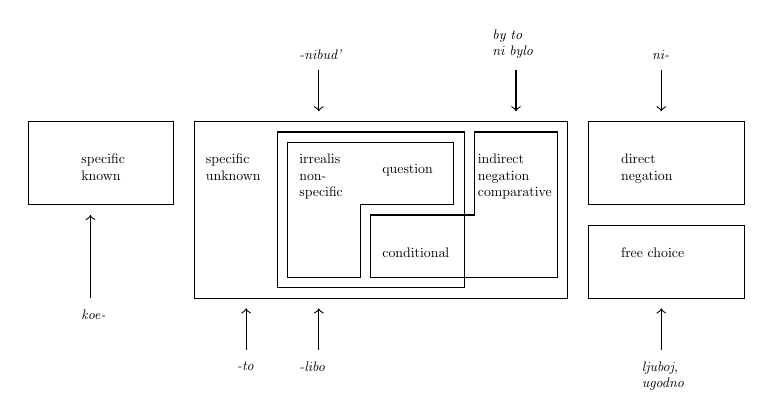
\begin{tikzpicture}[x=0.75pt,y=0.75pt,yscale=-1,xscale=1]
\centering 
    % boxes
    % 1 leftmost
    \draw (5,140) rectangle (75,100) ;
    % 2 elongated box
    \draw   (85,185) rectangle (265,100) ;
    % 3 box inside box 2
    \draw   (125,180) rectangle (215,105) ;
    % 4 top right
    \draw (275,140) rectangle (350,100) ;
    % 5 bottom right
    \draw (275,185) rectangle (350,150) ;
    
    % arrows 
    % arrow to box 1
    \draw[->] (35,185) -- (35,145);
    % arrow to box 2.topleft
    \draw[->]    (145,75) -- (145,95) ;
    % arrow to box 2.topright
    \draw[->]    (240,75) -- (240,95) ;
    % arrow to box 4
    \draw[->]    (310,75) -- (310,95) ;
    % arrow to box 5
    \draw[->]    (310,210) -- (310,190) ;
    % arrow to box 2.bottomright
    \draw[->]    (145,210) -- (145,190) ;
    % arrow to box 2.bottomleft
    \draw[->]    (110,210) -- (110,190) ;
    
    % L-shapes
    % left 
    \draw   (150,175) -- (150,175) -- (165,175) -- (165,140) -- (210,140) -- (210,120) -- (210,120) -- (210,120) -- (210,110) -- (130,110) -- (130,175) -- (150,175) -- cycle ;
    % right 
    \draw   (170,160) -- (170,160) -- (170,145) -- (220,145) -- (220,105) -- (240,105) -- (240,105) -- (240,105) -- (260,105) -- (260,175) -- (170,175) -- (170,160) -- cycle ;
    
    
    % Text
    % text inside boxes
    \draw (30,115) node [anchor=north west][inner sep=0.75pt]  [xscale=0.5,yscale=0.5] [align=left] {specific\\known};
    \draw (90,115) node [anchor=north west][inner sep=0.75pt]  [xscale=0.5,yscale=0.5] [align=left] {specific\\unknown};
    \draw (221,115) node [anchor=north west][inner sep=0.75pt]  [xscale=0.5,yscale=0.5] [align=left] {indirect\\negation\\comparative};
    \draw (135,115) node [anchor=north west][inner sep=0.75pt]  [xscale=0.5,yscale=0.5] [align=left] {irrealis\\non-\\specific};
    \draw (290,115) node [anchor=north west][inner sep=0.75pt]  [xscale=0.5,yscale=0.5] [align=left] {direct\\negation};
    \draw (290,160) node [anchor=north west][inner sep=0.75pt]  [xscale=0.5,yscale=0.5] [align=left] {free choice};
    \draw (175,160) node [anchor=north west][inner sep=0.75pt]  [xscale=0.5,yscale=0.5] [align=left] {conditional};
    \draw (175,120) node [anchor=north west][inner sep=0.75pt]  [xscale=0.5,yscale=0.5] [align=left] {question};
    % text outside boxes
    \draw (30,190) node [anchor=north west][inner sep=0.75pt]  [xscale=0.5,yscale=0.5] [align=left] {\textit{koe-}};
    \draw (135,65) node [anchor=north west][inner sep=0.75pt]  [xscale=0.5,yscale=0.5] [align=left] {\textit{-nibud'}};
    \draw (228,55) node [anchor=north west][inner sep=0.75pt]  [xscale=0.5,yscale=0.5] [align=left] {\textit{by to}\\ \textit{ni bylo}};
    \draw (305,65) node [anchor=north west][inner sep=0.75pt]  [xscale=0.5,yscale=0.5] [align=left] {\textit{ni-}};
    \draw (300,215) node [anchor=north west][inner sep=0.75pt]  [xscale=0.5,yscale=0.5] [align=left] {\textit{ljuboj},\\ \textit{ugodno}};
    \draw (135,215) node [anchor=north west][inner sep=0.75pt]  [xscale=0.5,yscale=0.5] [align=left] {\textit{-libo}};
    \draw (105,215) node [anchor=north west][inner sep=0.75pt]  [xscale=0.5,yscale=0.5] [align=left] {\textit{-to}};
\end{tikzpicture}
\label{fig:schemaähnlichkeiten}
\caption{Indefinitpronomen und -adverbialia des Russischen in Analogie zu dem Schema von \citet{Haspelmath1993}}
\end{figure}
\fi 


Die folgenden russischen Beispiele illustrieren das Schema und sind in ähnlicher Weise wie in \citet[264ff.]{Haspelmath1993} zusammengestellt.\footnote{Siehe auch die bei \citet[264]{Haspelmath1993} für die Distribution und Etymologie der Aus\-drucks\-rei\-hen der russischen Indefiniteinheiten angeführte relevante Literatur.}\textsuperscript{,}\footnote{Die Herausgeber haben die Beispiele um Glossen und Übersetzungen ergänzt.} Sie geben ein treffendes Bild von der Kompliziertheit der Verwendungsbedingungen russischer Indefinita (s. auch \citealt{Ruzicka1973,Ruzicka2000}).

\ea \textsc{Specific known}\\
    \gll Ja vstretilas' koe s kem desjat' minut nazad. \\
    ich traf.\textsc{refl} \textsc{spec} mit wem zehn Minuten zuvor \\ 
    \glt `Ich habe mich mit jemandem vor zehn Minuten getroffen.'
\z 

\newpage
\ea \textsc{Specific unknown}\\
    \gll Kto-to postučal v dver'. \\
        wer-\textsc{spec} klopfte in Tür \\
    \glt `Jemand hat an der Tür geklopft.'
\z 

\ea \textsc{Irrealis nonspecific (Imperative/Future)}\\
 \ea  \gll Spojte nam kakoj-nibud' / kakoj-libo romans.\\
    sing.2\textsc{pl}.\textsc{imp} uns was:für:ein-irgend {} was:für:ein-irgend Romanze \\
  \glt  `Singen Sie uns irgendeine Romanze!'\\
\ex  \gll  My vstretimsja gde-nibud' / gde-libo.\\
        wir treffen.\textsc{refl} wo-irgend {} wo-irgend \\ 
  \glt  `Wir werden uns irgendwo treffen.'
\z 
\z

\ea \textsc{Question/Conditional}\\
\ea  \gll  Zvonil li mne kto-nibud' / kto-libo?\\
           anrief Q mich wer-irgend {} wer-irgend \\ 
    \glt `Hat mich irgendwer angerufen?'
 \ex   \gll Esli čto-nibud' / čto-libo slučitsja, ja skažu mame.\\
    wenn was-irgend {} was-irgend passiert.\textsc{refl} ich sage Mutter \\
  \glt  `Wenn irgendetwas passiert, sage ich es Mutter.'
\ex   \gll Esli ty uslyšiš' čto by to ni bylo, razbudi menja.\\
    wenn du hörst was \textsc{cond} das \textsc{neg} wäre weck.2\textsc{sg}.\textsc{imp} mich \\
   \glt `Wenn du etwas hörst, was es auch immer sei, weck mich!'
\z 
\z 

\ea \textsc{Comparative}\\
    \gll Zdes' prijatnee žit', čem gde-libo / gde by to ni bylo v mire. \\
    hier angenehmer leben als wo-irgend {} wo \textsc{cond} das \textsc{neg} wäre in Welt \\
    \glt `Hier lebt es sich angenehmer als irgendwo, wo es auch immer sei, in der Welt.'
\z 

\ea \textsc{Indirect negation}\\
    \gll bez kakoj-libo / kakoj by to ni bylo pomošči \\
    ohne was:für:eine-irgend {} was:für:eine \textsc{cond} das \textsc{neg} wäre Hilfe\\
    \glt `ohne jedwede Hilfe'
\z 

\ea \textsc{Direct negation}\\
    \gll Nikogda ja ne zabudu tebja. \\
    \textsc{neg}-wann ich \textsc{neg} vergesse dich \\
    \glt `Ich werde dich niemals vergessen.'
\z 

\ea \textsc{Free choice}\\
    \gll Ty možeš' kupit' ljubuju / kakuju ugodno knigu. \\
    du kannst kaufen beliebiges {} was:für:ein beliebt Buch \\
    \glt `Du kannst ein beliebiges Buch kaufen.'
\z 

\noindent \citet{Seliverstova1988} untersucht die Verwendungsbedingungen der mit den Partikeln \textit{to-, nibud'-} und \textit{ni-} gekennzeichneten Pronomen und Adverbiale. Dabei wird deutlich gemacht, daß die Wahl der Partikeln mit bestimmten Präsuppositionen bezüglich der Möglichkeit des Nichteintretens der betreffenden Situation, der Existenz des jeweiligen Aktanten bzw. der Existenz von Wahlmöglichkeiten aus einer vorausgesetzten Menge von Aktanten zusammenhängt und durch den Satzmodus, Tempus und Aspekt, Matrixprädikate, Satzadverbien, Negation und Quantoren beeinflusst wird.

Es ist eine anspruchsvolle Aufgabe, alle diese Faktoren in ein System von semantischen und pragmatischen Verträglichkeiten zu bringen (s. dazu \citealt{Blaszczak2000}, Kap. 5) und zu entscheiden, welche Bedeutungskomponenten der beteiligten Ausdrücke in der SF zu berücksichtigen sind und welche selektionellen Zusammenhänge in Gestalt von Bedeutungspostulaten zum Tragen kommen. Ein solches Programm liegt jenseits der hier verfolgten Fragestellungen. Dennoch erscheint es nicht abwegig, im Einklang mit \citeauthor{Haspelmath1993}s (\citeyear{Haspelmath1993}) Klassifizierungen und mit den empirischen Generalisierungen \citeauthor{Seliverstova1988}s (\citeyear{Seliverstova1988}) mindestens mit folgenden Unterscheidungen zu rechnen:\footnote{Möglicherweise ist für \REF{ex:02:komponenten-sf} folgende Äquivalenz anzunehmen:
    
    \ea (\textsc{non})$_\alpha\, [ y\, \textsc{kennen}\, x ] = \exists Q\, [(\textsc{non})_\alpha\, [ y\, \textsc{fähig-zu}$ \linebreak $\textsc{charakterisieren}\, ^\cap\, Q]\, \&\, [ Q x ]]$
    \z 
    \noindent wobei der Operator $^\cap$ ein Prädikat zu einem Individuum macht. Diese Äquivalenz erfaßt, was Kenntnis bzw. Unkenntnis eines Objekts beinhaltet. Vgl. \citeauthor{Ruzicka1973}s (\citeyear{Ruzicka1973}: 726ff.) Cha\-rak\-te\-ri\-sie\-rung der für die \textit{koe-} bzw. \textit{to-}Reihe typischen Verwendungsbedingungen.}

\ea Die Partikeln \textit{-to, nibud'} und \textit{ni-} und die von \citet{Seliverstova1988} nicht behandelten Partikeln \textit{-libo} und \textit{koe-} treten nur in indefiniten +w-Phrasen auf. Ich nehme an, daß D der betreffenden Basiswörter (\textit{kto} `wer', \textit{gde} `wo' etc.) die morphosyntaktische Kennzeichnung +w -def hat.
\z 

\ea Die Partikel \textit{ni-} induziert das Merkmal +neg, die Partikeln \textit{koe-} und \textit{-to} das Merkmal +spez(ifisch), die Partikeln \textit{-nibud'} und \textit{-libo} das Merkmal -spez.
\z 

\ea\label{ex:02:komponenten-sf} Als Komponenten der SF induzieren \textit{koe-} [ $y$ \textsc{kennen} $x$ ] und \textit{-to} \textsc{non} [$y$ \textsc{kennen} $x$ ], und zwar als Präsuppositionen bezüglich der Identifizierbarkeit des mit x anvisierten Referenten.
\z 

\noindent Inwieweit bei Bildungen mit \textit{-libo, -nibud', by to ni bylo, ugodno} und \textit{ljuboj} die Präsupposition $[\textsc{beliebig}\, x]$ im Spiel ist, lasse ich offen.
\citet[60ff., 74f.]{Seliverstova1988} führt zu diesem Unterschied zwischen den Partikeln \textit{-to} und \textit{-nibud'} aus, daß ein beispielsweise durch
\textit{kto-to} `jemand' benannter Aktant als ,,individualisiert, aber für den Sprecher als unbekannt charakterisiert wird'' (ebd., 61), während bei \textit{-nibud'} ,,die Vorstellung vermittelt wird, daß es für den Sprecher unwichtig, gleichgültig ist, wer (was) an dem Ereignis beteiligt ist'' (ebd., 62) (Übersetzungen -- I.Z.).\footnote{Ich vernachlässige hier die von \citet{Seliverstova1988} an verschiedenen Stellen deutlich gemachten feinen Unterschiede bei der Verwendung von \textit{ljuboj/kto ugodno} `jeder beliebige' und von Bildungen mit \textit{-nibud'}, wobei jeweils besondere Präsuppositionen im Spiel sind. Ebenso lasse ich Bedeutungsnuancen beiseite, die zwischen Bildungen mit \textit{-to} bzw. \textit{-nibud'} im Ver\-gleich zu den Entsprechungen mit \textit{ni-} in Negationskontexten bestehen (s. \citealt[97ff.]{Seliverstova1988}). Wie stark auch Fragen des Quantorenskopus zu berücksichtigen sind, denen \citeauthor{Seliverstova1988} nicht systematisch nachgeht, mag folgendes Beispiel (ebd.: 93) andeuten:

\ea
\gll Ljuboj čelovek vsegda čem-to lučše kogo-to drugogo.\\
beliebiger Mensch immer was.\textsc{ins}-\textsc{spec} besser wer.\textsc{gen}-\textsc{spec} ander.\textsc{gen} \\
\glt ‘Jeder Mensch ist durch etwas besser als jemand anderes.’
\z 
}

Wir werden sehen, wie die von mir hier vorgeschlagenen morpho\-syntak\-tisch\-en Kennzeichnungen und Bedeutungskomponenten sich in die Struktur der zu analysierenden indefiniten Pronomen und Adverbiale einordnen.

\citet{Paduceva1985} klassifiziert pronominale und nichtpronominale Substantivgruppen hinsichtlich ihres Referenztyps in prädikative, definite, indefinite mit schwacher Bestimmtheit bzw. ohne schwache Bestimmtheit und gänzlich indefinite. (\ref{ex:02:Petrovic})--(\ref{ex:02:gazeta}) enthalten durch Kursivsetzung gekennzeichnete Beispiele für diese Einteilung.

\ea\label{ex:02:Petrovic}
\gll Anton Petrovič \textit{chorošij} \textit{učitel'}.\\
Anton Petrovič  guter Lehrer\\
\glt ‘Anton Petrovič ist ein guter Lehrer.’
\z 

\ea\label{ex:02:malcik}
\gll \textit{\.{E}tot} \textit{mal'čik}  bolen.\\
dieser Junge krank.\\
\glt ‘Dieser Junge ist krank.’
\z 

\ea\label{ex:02:prines}
\gll Ja tebe \textit{koe-čto} prines.\\
ich dir \textsc{spec}-was mitbrachte\\
\glt ‘Ich habe dir etwas mitgebracht.’
\z 

\ea\label{ex:02:poet}
\gll \textit{Kto-to} poet.\\
wer-\textsc{spec} singt \\
\glt ‘Jemand singt.’
\z 

\ea\label{ex:02:gazeta}
\gll Kupi \textit{kakuju-nibud'} \textit{gazetu}.\\
kauf.2\textsc{sg}.\textsc{imp} was:für:eine-irgend Zeitung \\
\glt ‘Kaufe irgendeine Zeitung!’
\z 

\noindent Nichtprädikative Substantivgruppen bestehen in der Regel aus einem oder auch mehreren sogenannten Aktualisatoren und der Deskription des Referenten. Zu den Aktualisatoren zählt \citet{Paduceva1985} -- ohne genaue morphosyntaktische Kategorisierungen anzugeben -- Determinatoren wie \textit{\.{e}tot} `dieser', Quantoren wie \textit{každyj} `jeder' und auch Numeralia wie \textit{mnogie} `viele' und \textit{dva} `zwei'. Pronomen wie \textit{koe-čto} `etwas', \textit{kto-to} `jemand', \textit{\.{e}to} `das', \textit{on} `er' gelten als Aktualisator ohne Deskription des Referenten.\footnote{\citet[154ff.]{Peskovskij1956} betont, daß den Pronomen und den pronominalen Adverbien keine konkrete gegenständliche Bedeutung zukommt und daß ihr Bedeutungsgehalt höchst abstrakt ist.} Eine morphosyntaktische oder se\-man\-ti\-sche Dekomposition der Pronomen wird nicht vorgenommen. Damit bleiben die angegebenen sehr subtilen Bedeutungs- und Verwendungsbesonderheiten der von \citeauthor{Paduceva1985} untersuchten Ausdrücke ohne genaue Zuordnung zu den beteiligten Formativen.

Ich nehme für \textit{koe-} und \textit{to-} die in (\ref{ex:02:komponenten-sf}) angegebenen Präsuppositionen an. Weitere semantische Unterscheidungen, z.B. zwischen Bildungen mit \textit{-libo} und \textit{-nibud'}, müssen ergänzt werden. Es ist auch zu klären, wie die einzelnen Kontextgegebenheiten, die das Auftreten der verschiedenen Indefinitphrasen bedingen (s. dazu \citealt{zi02:Isacenko1962,Dahl1970,Krizkova1971,Ruzicka1973,Ruzicka2000,Paduceva1985,Seliverstova1988,Haspelmath1993,Blaszczak2000}), in der Laut-Be\-deu\-tungs-Zu\-ord\-nung zu erfassen sind. Ich nehme an, daß für diese Kompatibi\-li\-täten auf der Ebene der Konzeptuellen Struktur entsprechende Bedeutungs\-po\-stu\-la\-te wirksam sind, die auf Gegebenheiten der durch die Grammatik determinierten SF der Konstruktionen zurückgreifen. Hier kommt es mir nur auf die Art der Installierung der betreffenden Informationen in die Bedeutungsstruktur der pronominalen Ausdrücke an.

Was die morphosyntaktische Kategorisierung der mit den einzelnen Partikeln gekennzeichneten Pronomen und Adverbiale angeht, nehme ich für D folgende Merkmalverteilung an:

%\ea\label{ex:02:merkmale}
%    \begin{tabularx}{.5\textwidth}{lrrrr}
%                                & w & def   & spez  & neg\\
%koe-                            & + & -     & +     & - \\
%-to                             & + & -     & +     & - \\
%-nibud'/-libo/ by to ni bylo    & + & -     & -     & - \\
%ni-                             & + & -     & -     & + \\
%$\varnothing$                   & - &       &       & - \\
%    \end{tabularx}
%\z 

\begin{table}
\caption{Merkmalverteilung für D}
\label{tab:zi02:1}
\begin{tabular}{lcccc}
\lsptoprule
        &w  &def    &spez   &neg\\
\midrule
\textit{koe-}   &$+$    &$-$    &$+$    &$-$\\
\textit{-to}    &$+$    &$-$    &$+$    &$-$\\                       \textit{-nibud'/-libo/ by to ni bylo}  &$+$    &$-$    &$-$    &$-$\\   
\textit{ni-}    &$+$    &$-$    &$-$    &$+$\\                       $\varnothing$  &$-$    &    &    &$-$\\ 
\lspbottomrule
\end{tabular}
\end{table}

\iffalse
\ea\label{ex:02:merkmale}
\begin{tabbing}
 \hspace{5cm}                    \= w \hspace{.5cm}   \= def \hspace{.5cm} \= spez \hspace{.5cm}    \= neg \\
koe-                            \> +                \> -                \> +                    \> - \\
-to                             \> +                \> -                \> +                    \> - \\
-nibud'/-libo/ by to ni bylo    \> +                \> -                \> -                    \> - \\
ni-                             \> +                \> -                \> -                    \> + \\
$\varnothing$                   \> -                \>                  \>                      \> - \\
\end{tabbing}
\z 

\fi 

%\noindent 
Alle durch die angegebenen Partikeln gebildeten komplexen Pronomen und Proadverbialia basieren auf \textit{k}-Wörtern. Sie haben in D die Merkmale $+$w $-$def. Es sind spezifisch bzw. unspezifisch referierende indefinite Ausdrücke. Der Nullartikel, den ich in Tabelle \ref{tab:zi02:1} zum Vergleich anführe, erhält seine Interpretation kontextabhängig und kann eine Substantivgruppe als definite bzw. indefinite spezifisch oder unspezifisch referierende Einheit qualifizieren (s. \citealt{Steube.Spaeth1998}).

Mit spezifisch referierenden Substantivgruppen ist die Präsupposition verbunden, daß das betreffende Objekt in der jeweils gegebenen Welt existiert.\footnote{\citet{Ruzicka1973} spricht von objektiver Identifikation, die für die Bildungen mit \textit{koe-} und \textit{to-} maßgebend ist.} Durch diese Präsuppositionen unterscheiden sich Bildungen mit \textit{-to} bzw. mit \textit{-nibud'} deutlich, wie \citeauthor{Paduceva1985}s (\citeyear{Paduceva1985}: 220) Beispiel andeutet:

\ea\label{ex:02:kislenkogo}
\gll Mne xočetsja čego-to / čego-nibud' kislen'kogo.\\
mir möchte.\textsc{refl} was.\textsc{gen}-\textsc{spec} {} was.\textsc{gen}-irgend Saures.\textsc{gen} \\
\glt ‘Ich möchte etwas / irgendetwas Saures.’ 
\z 

\noindent Die mit \textit{-to} gebildete Phrase referiert spezifisch, die mit \textit{-nibud'} gebildete un\-spe\-zi\-fisch (siehe Tabelle \ref{tab:zi02:1}). Das ist der einzige in (\ref{ex:02:kislenkogo}) zwischen den beiden Sätzen signali\-sierte Unterschied. Sind in LF noch irgendwelche Umformungen nötig, um für die SF zu den nötigen Unterscheidungen zu kommen? Ich muß in dieser Arbeit offenlassen, wie sich das morphosyntaktische Merkmal $\pm$spez auf die LF und die SF der betreffenden Sätze auswirkt.

\subsubsection{Lexikalische Bausteine der Analyse}\label{sec:zi02:indefinit-2}
Im Folgenden werden für einige russische Indefinitpronomen und -adverbialia die Grundannahmen meines Analysevorschlags weiter verdeutlicht und Lexi\-kon\-ein\-trä\-ge für die beteiligten Formative vorgeschlagen. Es wird sich zeigen, daß ich Indefinitphrasen grundsätzlich als lokal in D existenzquantifizierte Einheiten ansehe und für Indefinita nicht wie \textcite{Heim1982}, \textcite{Diesing1992} und \mbox{\citet{Blaszczak2000}} mit ungebundenen Variablen und besonderen Regeln der existential closure rechne.

Wie schon in den Abschnitten \ref{sec:zi02:relativ} und \ref{sec:zi02:interrogativ} dargelegt wurde, nehme ich an, daß das Stützmorphem der Pronomen, das semantisch den Restriktor charakterisiert, als N unter NP erzeugt wird und in der PF durch Kopfbewegung zum Adjunkt von D wird. Wie bei allen nichtrelationalen N handelt es sich um einstellige Prädikatausdrücke. Vgl. die folgenden Lexikoneinträge: \enlargethispage{1\baselineskip}

\ea\label{ex:02:lex-null}
    \ea /\varnothing/
    \ex $-$V $+$N
    \ex $+$w \_
    \ex $\lambda x\, [\,\cnst{person} \, x]\, \textrm{mit}\, \cnst{person} \in \langle e,t\rangle$
\z\z 

\ea\label{ex:02:lex-de}
    \ea /de/
    \ex $-$V $+$N $+$adv
    \ex $+$w resp. $+$Q resp. $+$def $-$prox \_\_
    \ex $\lambda x\, [\,\cnst{ORT}\, x\,]\, \textrm{mit}\, \cnst{ORT} \in \langle e,t\rangle$
\z\z 

\ea\label{ex:02:lex-gda}
    \ea /gda/
    \ex $-$V $+$N $+$adv
    \ex $+$w resp. $+$Q resp. $+$def $-$prox / $+$neutr \_
    \ex $\lambda x\, [\,\cnst{ZEIT}\, x\,]\, \textrm{mit}\, \cnst{ZEIT} \in \langle e,t\rangle$
\z\z 

\noindent Die Lexikoneinträge (\ref{ex:02:lex-null})--(\ref{ex:02:lex-gda}) charakterisieren die Stützmorpheme von \textit{kto} `wer', \textit{gde} `wo' und \textit{kogda} `wann'. Dabei ist in (b) die morphosyntaktische Kate\-go\-ri\-sie\-rung des Formativs angegeben. $+$adv kennzeichnet -- Ns mit adverbiell zu interpretierender Kasusendung vergleichbar -- die betreffenden adverbiellen Stützmorpheme. (c) sind Anforderungen an die oberflächenstrukturelle Nachbarschaft des Formativs und damit die Grundlage für Kopfbewegung des N nach D in PF. Und zwar verlangen diese gebundenen Morpheme eine gegebenenfalls flektierte $+$w-, $+$Q- bzw. $+$def $-$prox-Einheit als wortstrukturellen Nachbarn.\footnote{\label{fn:18} Einschlägigen etymologischen Wörterbüchern wie \citet{Preobrazenskij1958} und \citet{Vasmer1964} ist -- bei aller Nichtübereinstimmung und Vorsichtigkeit der Auskünfte -- zu den hier zu analysierenden pronominalen Adverbialia zu entnehmen, daß es sich um morphosyntaktisch komplexe Ausdrücke handelt, die sich aus einem pronominalen Bestandteil (\textit{k-, t-, v(e)s'-, \mbox{in-})} und suffixartigen Einheiten (\textit{-de, -gda, -k, -da, -du}) zusammensetzen. Warum dabei einmal die nach maskulinem Genus und dann wieder nach Femininum bzw. Neutrum Singular Nomi\-nativ bzw. Akkusativ aussehende pronominale Form (also z.B. \textit{k-} in \textit{gde} `wo', \textit{ka-} in \textit{kak} `wie', \textit{ko-} in \textit{kogda} `wann', \textit{ku-} in \textit{kuda} `wohin' und \textit{vsju-} in \textit{vsjudu} `überall') verwendet wird, bleibt offen. Ich nehme -- im Sinne von Volksetymologie -- an, daß eine Art Kongruenz zwischen Determinator und Stütznomen vorliegt und kennzeichne die eine bestimmte Determinatorform selegierenden Formative entsprechend.} (d) charakterisiert die Bedeutung des Formativs. Sie dient als Restriktorprädikat.\footnote{Im Grunde genommen handelt es sich bei dem Bedeutungsbeitrag der Stützmorpheme um die sortale Charakterisierung des Wertebereichs der jeweiligen Variablen. Ich rechne diese Charakterisierung hier dem Restriktorteil von DP-Bedeutungen zu.}

An diese NP-Köpfe können Modifikatoren angeschlossen sein, die zusammen mit der N-Bedeutung ein komplexes Restriktorprädikat bilden. Ich deute das in (\ref{ex:02:kto-iz}) für \textit{kto iz vas} `wer von euch' an.\footnote{Zur Unifizierung von Prädikaten siehe \citet{Zimmermann1992} und \citet{Wunderlich1997b}.}

\ea\label{ex:02:kto-iz}
    \ea $[_\textrm{NP}\, [_\textrm{NP}\, [_\textrm{NP}\, \varnothing ]][_\textrm{PP}\, [_\textrm{P}\, \textrm{iz} ][_\textrm{DP}\, \textrm{vas}]]]$
    \ex $\lambda x\, [[\,\cnst{PERSON}\, x\,]\, \& \, \exists!y\, [[ y > 1]\, \&\, [\,\cnst{ADRESSAT} y\, ]] [x \subset y ]]$
\z\z 

\noindent Fundamental für meine Analyse ist die Kategorisierung der Determinatoren und die ihr zugeordnete Bedeutung des jeweiligen Formativs. Ich gebe einige Beispiele.

\ea\label{ex:02:47}
    \ea /t/
    \ex $+$D $+$def $-$prox $-$max
    \ex $\lambda P\, \lambda Q\, \exists! x\, [[ P x ]\, (\&\, [ \textsc{non}\, [\,\cnst{PROX}\, x\,]]) ][Q x]$
\z\z 

\ea\label{ex:02:48}
    \ea /k/
    \ex $+$Def $+$w $-$def $\alpha$max 
    \ex ($+$neg)$_{-\beta}\, [_\textrm{D}\, [_\textrm{D} \_\_ \textrm{(X)} ]\, \textrm{N} ]$
    \ex\label{ex:02:48d} $\lambda P_1\, \underset{\gamma spez}{(\lambda P_2)_\beta}\, \lambda Q \exists x [([P_2 \, x] :)_\beta [P_1 x]][Q x]$
\z\z 

\ea\label{ex:02:49}
    \ea /koe/
    \ex $+$spez
    \ex \_\_ $+$w $-$def $+$max
    \ex\label{ex:02:49d} $\lambda \textrm{x}\, [\,y\, \textsc{kennen}\, x\,]$
\z\z 

\ea\label{ex:02:50}
    \ea /to/
    \ex $+$spez
    \ex $+$w $-$def $+$max \_\_
    \ex\label{ex:02:50d} $\lambda x\, \textsc{non}\, [\,y\, \textsc{kennen}\, x\,]$
\z\z 

\ea\label{ex:02:51}
    \ea /ni/
    \ex $+$neg
    \ex \_\_ $+$w $-$def $+$max
    \ex\label{ex:02:51d} $\lambda x\, [x]$
\z\z 

\noindent (\ref{ex:02:47}) charakterisiert den Determinator \textit{tot} `der'/`jener', durch die mögliche Komponente NON [ PROX $x$] im Kontrast zu \textit{\.{e}tot} `dieser'.\footnote{Die Determinatoren \textit{tot} und \textit{\.{e}tot} weisen im Nominativ und Akkusativ Maskulinum Singular bedeutungsleere Erweiterungen auf. Zu den Besonderheiten der pronominalen Flexion siehe \citet{Zaliznja1977}.} (\ref{ex:02:48}) ist der grundlegende Determinator für Indefinitpronomen und -adverbialia. Er bindet die referentielle Argumentstelle der NP und führt eine Argumentstelle für die durch Partikeln und andere Zusätze ausgedrückte pragmatische Präsupposition ein, die in (\ref{ex:02:49d}) für \textit{koe-} und in (\ref{ex:02:50d}) für \textit{-to} expliziert ist. (\ref{ex:02:51}) liefert die Partikel \textit{ni-}, die für Negativpronomen und -adverbialia konstitutiv ist. Ich nehme an, daß durch (\ref{ex:02:48d}) und (\ref{ex:02:51d}) Negativpronomen und -adverbialia durch Existenzquantifizierung charakterisiert sind und gemäß einer dem Bindungsprinzip A vergleichbaren Vorschrift durch die Satznegation legitimiert werden (s. dazu \citealt{Progovac1994}; \citealt[Kap. 4]{Blaszczak1998,Blaszczak2000}).\footnote{Negativpronomen und -ad\-verbialia treten auch in Nomi\-na\-li\-sierungen auf, die durch den Negator \textit{ne-} präfigiert sind (s. dazu \citealt{Zimmermann1988}). Auf diese Fälle muß die Strukturvorschrift für die Legitimierung der \textit{ni}-Einheiten erweitert werden. Und zwar liegen semantisch alle Vorkommen von Negativpronomen und -ad\-ver\-bialia im Skopus der Negation. Für Nomi\-na\-li\-sierungen wie (\ref{ex:02:fn22}) bedeutet das, daß die Bedeutung des Präfixes \textit{ne-} erst auf der NP-Ebene wirksam werden kann.

\ea\label{ex:02:fn22}
    \gll nepoxožest' devočki ni v čem ni s kem iz sem'i \\
    Unähnlichkeit Mädchen.\textsc{gen} \textsc{neg} in was \textsc{neg} mit wem aus Familie \\ 
    \glt ‘Das Mädchen ist in nichts wem aus der Familie ähnlich.’
\z 

\noindent \citet[Kap. 5 und 6]{Blaszczak2000} macht fürs Polnische deutlich, daß die Negativpronomen und\linebreak {-adverbialia} lizensierende Negation ein vergleichsweise starker Negationsausdruck sein muß und daß die Lizensierung in der syntaktischen Derivation zyklisch -- von Phase zu Phase (s. \citealt{Chomsky1998,Chomsky1999}) -- erfolgt. Es ist ein Thema für sich, welche Nominalisierungen mit einem mit \textit{ne-} präfigierten deverbalen bzw. deadjektivischen Nomen in Kopffunktion als solche Phasen anzusehen sind und ob auch fürs Russische wie fürs Polnische mit syntaktisch deri\-vier\-ten Nominalisierungen zu rechnen ist.}

Ich sehe also den Determinator wie in (\ref{ex:02:47}) und (\ref{ex:02:48}) als Binder oder wie in (\ref{ex:02:lexikoneintrag-d}) als Blockierer der referentiellen Argumentstelle der NP an. Die bei den Indefinita im Russischen unerläßlichen Partikeln liefern pragmatische Präsuppositionen bzw. die Kennzeichnung einer DP als an die Negation gebunden.

Was an Bausteinen meiner Analyse noch ergänzt werden muß, ist die Adverbialisierung der pronominalen Adverbiale. Sie geschieht, wie schon im Abschnitt \ref{sec:zi02:relativ} illustriert wurde, als Einbettung in eine PP mit einer phonologisch leeren Präposition:

\ea\label{ex:02:52}
    \ea /\varnothing/
    \ex $-$V $-$N $+$adv
    \ex $\lambda\textfrak{R}\, \lambda y [\, \textfrak{R}\lambda x\, [y\, R\, x]]$ mit \textfrak{R} $\in \langle\langle e,t\rangle,t\rangle, R \in \langle e, \langle e,t\rangle\rangle$
    \z
\z 

\noindent Dabei ist $R$ ein zu spezifizierender Parameter für eine abstrakte Relation zwi\-schen $y$ und $x$, etwa für Enthaltensein. Das indefinite Adverbial \textit{koe-gde} `an einem bestimmten Ort' hat dann die folgende Repräsentation:\enlargethispage{2\baselineskip}

\ea 
    \ea $[_\textrm{PP}\, [_\textrm{P}\, \varnothing ][_\textrm{DP}\, [_\textrm{D}\, \textrm{koe}\, [_\textrm{D}\, \textrm{k} ]][_\textrm{NP}\, [_\textrm{N}\, \textrm{de} ]]]]$
    \ex $[_\textrm{PP}\, [_\textrm{P}\, \varnothing ][_\textrm{DP}\, [_\textrm{D}\, \textrm{koe}\, [_\textrm{D}\, [_\textrm{D}\, \textrm{k} ][_\textrm{N}\, \textrm{de}]]]]]$
    \ex $\lambda y\, \exists x\, [[\, z\, \textsc{kennen}\, x \,] : [\, \cnst{ORT}\, x \,]][\, y\, R\, x \,]$
    \z
\z 

\noindent Dabei ist (a) die LF, (b) die Eingabe in PF und (c) die SF des morphosyntaktisch und semantisch komplexen Ausdrucks.

Wenn eine phonologisch nichtleere Präposition mit einem Indefinitpronomen, das mit der Partikel \textit{koe-} oder \textit{ni-} beginnt, unmittelbar benachbart ist, erfolgt für \textit{koe-} fakultativ und für \textit{ni-} obligatorisch Voranstellung der Partikel vor die Präposition.\footnote{Siehe \citet[66, 76]{Zaliznja1977}: 
\ea
\gll ot koe-čego / koe ot čego\\
    von \textsc{spec}-was.\textsc{gen} {} \textsc{spec} von was.\textsc{gen}\\
\glt ‘von etwas’
\z 
\noindent Zum Ausbleiben der Metathese bei komplexen Präpositionen wie \textit{otnositel'no} `bezüglich', \textit{blagodarja} `dank' siehe \citet{Yadroff.Franks1999}.} Vgl. die folgenden \citet[164]{Isacenko1965} entnommenen Beispiele:

\ea
    \gll Koe-kto koe s kem koe-kodga koe o čem govoril.\\
    \textsc{spec}-wer \textsc{spec} mit wem \textsc{spec}-wann \textsc{spec} über was sprach \\
     \glt ‘Jemand hat mit jemandem einmal über etwas gesprochen.’
\z 

\ea
    \gll Nikto ni s kem nikogda ni o čem ne govoril.\\
    \textsc{neg}.wer \textsc{neg} mit wem \textsc{neg}.wann \textsc{neg} über was \textsc{neg} sprach \\
    \glt ‘Niemand hat mit niemandem nie über etwas gesprochen.’
\z 

\noindent Ich nehme an, daß es sich um eine Permutation auf der Ebene der PF handelt (zur historischen Entwicklung und zum Vergleich slawischer Sprachen bezüglich dieser Metathese s. \citealt{Billings1997}).


\subsection{Pronomen und Adverbialia mit Allquantifizierung}\label{sec:zi02:allquant}

Ich will nun noch einen Blick auf zwei Adverbiale werfen, in denen das Formativ \textit{v(e)s'} `alle' auftritt, \textit{vezde} `überall' und \textit{vsegda} `immer'. Zu den bereits angeführten Bestandteilen dieser Ausdrücke ist nur \textit{v(e)s'} zu ergänzen.

\ea\label{ex:02:56}
    \ea /v(e)s'/
    \ex $+$D $+$Q \textalpha max
    \ex\label{ex:02:56d} $\lambda P\, \lambda Q\, \forall x\, [\, P x \,][\, Q x \,]$
\z\z 

\noindent Das als Allquantor interpretierte Formativ kann als selbständiges Pronomen wie \textit{vse} `alle' oder wie in \textit{vse učeniki} `alle Schüler' verwendet werden oder als Komponente von Adverbialia auftreten.\footnote{Die Annahmen \citeauthor{Giusti1991}s (\citeyear{Giusti1991}) zur Kategorisierung von Quantorausdrücken und zu der entsprechenden Konstituentenstruktur von Substantivgruppen kann ich hier nicht diskutieren. Für \textit{v(e)s'} sind vermutlich zwei Bedeutungscharakterisierungen anzunehmen, die eine wie in (\ref{ex:02:56d}) für den Allquantor und die andere für Verwendungen wie in \textit{ves' den'} `den ganzen Tag'.} Für \textit{vezde} `überall' und \textit{vsegda} `immer' ergibt sich dann zusammen mit der Bedeutung der phonologisch leeren Präposition (s. (\ref{ex:02:52})) folgende SF:

\ea $\lambda y\, \forall x\, [\, \cnst{ORT/ZEIT}\, x\,] [\, y\, R\, x \,]$ 
\z 

\noindent Das sind Prädikate, die durch Argumentstellenunifizierung mit einem Modifikanden verbunden werden können, z.B. wie in (\ref{ex:02:58}) und (\ref{ex:02:59}).

\ea\label{ex:02:58}
    \gll Vezde suščestvuet besporjadok.\\
    überall existiert Unordnung\\
    \glt ‘Überall herrscht Unordnung.’
    
\z 

\ea\label{ex:02:59}
    \gll Boris  vsegda p'jan.\\
    Boris immer betrunken\\
    \glt ‘Boris ist immer betrunken.’
\z 

\noindent Bezüglich des Adverbs \textit{vsegda} ist zu berücksichtigen, daß es nach \citet[222ff.]{Paduceva1985} neben seiner temporalen Bedeutung auch einfach die Funktion eines Allquantors haben kann,\footnote{Zur Degenerierung des Restriktors siehe auch \citet[95ff.]{Acquaviva1995}. \citet[163]{Isacenko1965} meint, daß die Bedeutung einiger Pronomen und pronominaler Adverbien sich ganz in der Funktion als All- bzw. Existenzoperator erschöpft. Er rechnet auch \textit{vsegda} `immer' dazu.} mit Bezug auf Situationen bzw. auf beliebige Objekte. Vgl. die aus \citet[231]{Paduceva1985} entlehnten Beispiele, wobei die allquantifizierten Phrasen kursiviert sind:

\ea
    \gll Summa \textit{dvux} \textit{nečetnyx} \textit{čisel}  vsegda četna.\\
    Summe zwei.\textsc{gen} ungerade.\textsc{gen} Zahlen.\textsc{gen} immer gerade\\
    \glt ‘Die Summe zweier ungerader Zahlen ist immer gerade.’
\z 

\ea
    \gll Počti vsegda \textit{talant} poraboščaet svoego obladatelja.\\
    fast immer Talent versklavt seinen Besitzer\\
    \glt ‘Ein Talent versklavt fast immer seinen Besitzer.’
\z 

\noindent Hier stellen sich einige Fragen: Wenn es sich bei \textit{vsegda} tatsächlich um einen reinen Allquantor ohne Bezug auf Zeit handelt, ist wohl ein Bedeutungsschwund anzunehmen, so daß die temporale Wertebereichscharakterisierung als annulliert bzw. auf einen universellen Wertebereich erweitert angesehen werden muß. Wie ist das im Lexikoneintrag für \textit{vsegda} zu berücksichtigen? Padučeva rechnet einfach mit mehreren \textit{vsegda}. Ferner ist zu fragen, wie Syntax, Morphologie und Semantik in solchen Fällen zusammenwirken. Jedenfalls zeigen die Beispiele deutlich genug, daß morphosyntaktische Oberflächenstruktur und semantische Strukturbildung relativ weit auseinandergehen können. Ich muß es bei dieser Feststellung belassen, auch wenn ich dem Ideal ``Ein Formativ -- eine Bedeutung'' anhänge und es auch wie bei \textit{vsegda} erst einmal nicht aufgeben möchte. Wieso sollte es für Beispiele wie oben nicht eine mit der Paraphrase `es ist fast immer so, daß' korrespondierende Lösung geben?

\subsection{Die Reichweite der Analyse}\label{sec:zi02:reichweite}

Meine Analysevorschläge für einige russische Pronomen und Proadverbialia, die als Glieder in Proportionalgleichungen oder in Reihen wie in Tabelle \ref{tab:reihen} und in Beispiel (\ref{ex:02:k-partikeln}) eine Ahnung der Sprecher und Hörer von der morphosyntaktischen und semantischen De\-kom\-po\-nier\-bar\-keit der Wörter durchscheinen lassen, erhebt durchaus den An\-spruch, im Prinzip nicht nur für das Russische gültig zu sein. Andererseits wirft die Analyse die Frage auf, für welche Pronomen und Proadverbialia des Rus\-si\-schen sie anzuwenden ist.

Wie steht es z.B. mit \textit{zdes'} `hier', das aus dem Determinator \textit{s'}, dem Stützmorphem \textit{de} mit lokaler Bedeutung und wohl einer Partikel \textit{s'} zusammengesetzt ist?\footnote{Siehe \citet[II 89f.]{Vasmer1964}.} Wie ist \textit{skol'ko} `wieviel' zu analysieren, wenn überhaupt?\footnote{Vermutlich ist \textit{skol'ko} `wieviel' auf die Präposition \textit{s} `nahe', ein pronominales Element \textit{k}, ein Stützmorphem \textit{ol'} `Quantum' und ein Suffix \textit{ko} zurückzuführen. Siehe \citet[335]{Preobrazenskij1958}, \citet[III 647]{Vasmer1964}.} Oder wie verfährt man mit \textit{vsjudu v parke} `überall im Park', wo \textit{v parke} als restringierender Modifikator mit der Beutungsstruktur von \textit{vsjudu} passend zusammengefügt werden muß? Ich stelle für dieses Beispiel drei mögliche Analysen zur Diskussion, um zu verdeutlichen, was die Laut-Bedeutungs-Zuordnung leisten muß.

Analyse A1 folgt den bisher erläuterten Verfahren:\footnote{Zur Analyse von \textit{vsjudu} `überall' siehe \citet[102]{Preobrazenskij1958} und \citet[364]{Vasmer1964}.}

\ea\label{ex:02:62}
    \ea\label{ex:02:62a} $[_\textrm{PP}\, [_\textrm{P}\, \varnothing] [_\textrm{DP}\, [_\textrm{D}\, \textrm{vsju}] [_\textrm{NP}\, [_\textrm{NP}\, [_\textrm{N}\, \textrm{du}]] [_\textrm{PP}\, [_\textrm{P}\, \textrm{v}\, [_\textrm{DP}\, \textrm{parke}]]]]]$
    \ex\label{ex:02:62b} $[_\textrm{PP}\, [_\textrm{P}\, \varnothing] [_\textrm{DP}\, [_\textrm{D}\, [_\textrm{D}\, \textrm{vsju} ][_\textrm{N}\, \textrm{du}]] [_\textrm{PP}\, [_\textrm{P}\, \textrm{v}\,] [_\textrm{DP}\, \textrm{parke}]]]]$
    \ex\label{ex:02:62c} $\lambda \textfrak{R}\, \lambda y\, [\textfrak{R} \lambda y\, [\, y\, R\, x\,]] (\lambda P\, \lambda Q\, \forall x\, [\, P x \,][\, Q x \,]\linebreak
    (\lambda P\, \lambda Q\, \lambda x\, [\, P x \,]\, \& \,[\, Q x \,]\, (\lambda z\, [\, z \subset \textsc{in park}\, ]) 
    (\lambda x\, [\, \cnst{ORT}\, x \,] )))\linebreak
    = \lambda y\, \forall x [[ \cnst{ORT}\, x ]\, \& \,[\, x \subset \textsc{in park} \,]][\, y\, R\, x \,]$
    \z
\z 

\noindent (a) repräsentiert die der SF (c) zugrunde liegende LF. (b) ist die Eingabe in die PF. Bei der semantischen Amalgamierung verknüpft ein Template den Modifikator \textit{v parke} und den Modifikand, das adverbielle gebundene Morphem \textit{du}.\footnote{Zur Modifikation siehe \citet{Zimmermann1992} und \citet{Wunderlich1997b}. Der Modifikator \textit{v parke} `im Park' ist in (\ref{ex:02:62c}) vereinfacht repräsentiert.}

Wenn man auf die in (\ref{ex:02:62a}) gegebene syntaktische Dekomposition verzichtet und Pronomen und Proadverbialia unter D erzeugt wie in (\ref{ex:02:62b}) und dennoch den Modifikator wie in (\ref{ex:02:62c}) -- als restringierende Ergänzung -- integrieren will, muß dem Determinator -- hier \textit{vsju}, eine von \textit{du} selegierte Form von \textit{v(e)s'} -- eine fakultative Argumentstelle für den Modifikator beigegeben werden (vgl. (\ref{ex:02:63}) und (\ref{ex:02:56})):\footnote{Siehe Anm. \ref{fn:18}.}

\ea\label{ex:02:63}
    \ea /v(e)s'/
    \ex $+$D $+$Q \textalpha max
    \ex $\lambda P_1\, (\lambda P_2)\, \lambda Q\, \forall x\, [[P_1\, x]\, (\&\, [P_2\, x\,])] [\, Q x \,]$
    \z
\z 

\noindent Entsprechend wäre bei anderen hier betrachteten Determinatoren zu verfahren. Diese Analyse A2 läuft darauf hinaus, daß die Integration von Modifikatoren hier auf besondere -- von nichtpronominalen DPs und PPs verschiedene -- Weise erfolgt (vgl. \textit{na vsex mestax v parke} `an allen Stellen im Park').

Eine dritte Version A3 verzichtet auf die Dekomposition des pronominalen Adverbs und erzeugt \textit{vsjudu} direkt als intransitive P wie in (\ref{ex:02:64}).

\ea\label{ex:02:64} $[_\textrm{PP}\, [_\textrm{P}\, \textrm{vsjudu}] [_\textrm{PP}\, [_\textrm{P}\, \textrm{v}\,] [_\textrm{DP}\, \textrm{parke}]]]$ \z

\noindent Dann muß die Argumentstelle für den fakultativen Modifikator der Adverbbedeutung hinzugefügt werden wie in (\ref{ex:02:65}).

\ea\label{ex:02:65}
    \ea /vsjudu/
    \ex $-$V $-$N
    \ex $(\lambda Q)\, \lambda y\, \forall x\, [[\, \cnst{ORT}\, x \,]\, (\&\, [\, Q x \,])] [\, y\, R\, x \,]$
\z\z 

\noindent Diese Version garantiert zwar, daß sich die gleiche SF wie bei A1 und A2 des Beispiels ergibt, sie verzichtet aber auf jegliche morphosyntaktische Analyse des pronominalen Adverbs.

Ich habe damit angedeutet, wie verschiedene Dekompositionsverfahren aussehen können. Es scheint mir bei dem betrachteten Fall und im Prinzip durchaus möglich, daß ein Sprachlerner in verschiedenen Phasen des Spracherwerbs unterschiedliche Analysen macht, je nachdem welche paradigmatischen und syntagmatischen Zusammenhänge der Laut-Bedeutungs-Zuordnung er erkennt.

In diesem Sinn betrachte ich die morphosyntaktische und semantische Dekomponierbarkeit von Pronomen und Proadverbialia als etwas Relatives. Jedoch ist der Sinn für Durchsichtigkeit und Motiviertheit von Zeichen -- so meine ich -- nicht zu unterschätzen. Und es ist auch in relativ geschlossenen Gruppen von Wörtern, wie sie Pronomen und Proadverbialia darstellen, mit Systematik zu rechnen.
    
\subsection{Die Aussagekraft von Morphologiekonzepten mit morphologischen Korrespondenzregeln}\label{sec:zi02:alternative}

Die vorstehende Analyse\footnote{Zu diesem als Appendix zu verstehenden Abschnitt hat mich die Diskussion mit Marga Reis veranlaßt.} geht davon aus, daß die hier betrachteten Pronomen und Proadverbialia morphosyntaktisch und semantisch analysierbar sind, und bezieht die beteiligten Formative durch entsprechende Informationen in den Lexi\-kon\-ein\-trä\-gen und durch syntaktische Kopf-zu-Kopf-Bewegung systematisch auf\-ein\-an\-der. Dabei wurde auch berücksichtigt, daß restringierende Modi\-fi\-ka\-tor\-phra\-sen wie in \textit{vsjudu v parke} `überall im Park' genauso mit dem Modifikandum verknüpft sind wie in vergleichbaren PPs, z.B. in \textit{na vsex mestax v parke} `an allen Orten im Park'. Es wurde angenommen, daß sich restringierende Modifikatoren an den Restriktor der betreffenden Ausdrücke anschließen, mindestens in der semantischen Repräsentation (vgl. die Analysevarianten im Abschnitt \ref{sec:zi02:reichweite}.).

Ich will nun noch zu skizzieren versuchen, wie in einem Morphologiekonzept, das Wortformen zueinander in Beziehung setzt, ohne eine morphosyntaktische Analyse in Morpheme vorzunehmen (s. \citealt{Matthews1991}, Abschn. 10), die bestehenden Form-Inhalt-Bezüge erfaßt werden könnten. Dazu gehen wir von der in Abschnitt \ref{sec:zi02:reichweite} für \textit{vsjudu} `überall' angedeuteten Analyse A3 aus.

Es handelt sich bei dieser Lokalangabe um eine intransitive Präposition mit der lexikalischen Kategorisierung $-$V$-$N. Dieses Adverb korrespondiert sys\-te\-ma\-tisch mit den Adverbien \textit{vezde} `überall' und \textit{vsegda} `immer' (zu \textit{vsjako} `auf jede Weise' s. Anm. \ref{fn:1}). Und die Adverbien ihrerseits korrespondieren mit dem Quantor \textit{v(e)s'/vse} `ganz'/`alle', der der Kategorie $+$D$+$Q angehört und im Instrumental Singular Maskulinum bzw. Neutrum und im Plural mit \textit{e} anlautende Flexive aufweist. Man könnte sagen, daß auch die adverbiellen Ausdrücke zum Paradigma von \textit{v(e)s'} gehören und daß alle betreffenden Wortformen durch `$\leftrightarrow$' -- paradigmatische Zusammengehörigkeit symbolisierend (vgl. \citealt{Jackendoff1975}) -- aufeinander bezogen werden. 

(\ref{ex:02:66}) ist der Lexikoneintrag für \textit{v(e)s'} (vgl. (\ref{ex:02:56})), (\ref{ex:02:67}) gibt morphologische Kor\-res\-pon\-denz\-re\-geln an, die Wortformen von \textit{v(e)s'}, aber auch die von \textit{tot} `der'/`jen\-er' verallgemeinernd aufeinander beziehen. Es besteht Kovariation zwi\-schen der PF und der MSC, die SF variiert nicht.

\ea\label{ex:02:66}
    /v(e)s'/ \\
    $+$D $+$Q \\
    $+$e-Flexive\\
    $-$neutr $-$fem\\
    $-$plur\\
    $\fracx{+\textrm{nom}}{+\textrm{acc}}$ \\
    $\lambda P\, \lambda Q\, \forall x\, [\, P x \,] [\, Q x \,]$
\z 

%\ea\label{ex:02:67}
%\begin{tabularx}{\textwidth}{XXXXXXX}
%/X/                                    &                   & /X+o/                                  &                   & /X+e/                                  &                   &       \\
%$+$D                                   &                   & $+$D                                   &                   & $+$D                                   &                   &       \\
%$+$e-Flexive                           &                   & $+$e-Flexive                           &                   & $+$e-Flexive                           &                   &       \\
%$-$neutr $-$fem                        & $\leftrightarrow$ & $+$neutr $-$fem                        & $\leftrightarrow$ &                                        & $\leftrightarrow$ & \dots \\
%$-$plur                                &                   & $-$plur                                &                   & $+$plur                                &                   &       \\
%$\fracx{+\textrm{nom}}{+\textrm{acc}}$ &                   & $\fracx{+\textrm{nom}}{+\textrm{acc}}$ &                   & $\fracx{+\textrm{nom}}{+\textrm{acc}}$ &                   &       \\
%Y                                      &                   & Y                                      &                   & Y                                      &                   &      
%\end{tabularx}
%\z 

\newpage
\ea\label{ex:02:67}
\begin{tabbing}
    /X/  \hspace{2cm}                                  \= \hspace{1cm}                  \= /X+o/ \hspace{2cm}                                 \= \hspace{1cm}                   \= /X+e/ \hspace{1cm}                                 \= \hspace{1cm}                   \=       \\
$+$D                                   \>                   \> $+$D                                   \>                   \> $+$D                                   \>                   \>       \\
$+$e-Flexive                           \>                   \> $+$e-Flexive                           \>                   \> $+$e-Flexive                           \>                   \>       \\
$-$neutr $-$fem                        \> $\leftrightarrow$ \> $+$neutr $-$fem                        \> $\leftrightarrow$ \>                                        \> $\leftrightarrow$ \> \dots \\
$-$plur                                \>                   \> $-$plur                                \>                   \> $+$plur                                \>                   \>       \\
$\fracx{+\textrm{nom}}{+\textrm{acc}}$ \>                   \> $\fracx{+\textrm{nom}}{+\textrm{acc}}$ \>                   \> $\fracx{+\textrm{nom}}{+\textrm{acc}}$ \>                   \>       \\
Y                                      \>                   \> Y                                      \>                   \> Y                                      \>                   \> \\
\end{tabbing}
\z

\noindent (\ref{ex:02:68}) setzt \textit{v(e)s'} zu dem dieses Formativ enthaltenden Adverb \textit{vezde} `überall' in Beziehung. Die aufgegliederte SF von \textit{vezde} in (\ref{ex:02:68}) (vgl. Anm. \ref{fn:10}) macht die semantische Korrespondenz von \textit{v(e)s'} und \textit{vezde} transparent. Morphosyntaktische Korrespondenzen bleiben hier allerdings -- im Gegensatz zu den Analysen A1 und A2 in Abschnitt \ref{sec:zi02:reichweite} -- verborgen, unexpliziert. Auch die in A1 und A2 erfaßten Zusammenhänge zwischen den Bedeutungskomponenten des Adverbs und phrasen- bzw. wortstrukturellen Gegebenheiten vergleichbarer Ausdrücke bleiben im Dunkeln.

%\ea\label{ex:02:68}
%\begin{tabularx}{.8\textwidth}{XXX}
%/v(e)s'/                                      &                   &  /v(e)s'$+$de/                                                        \\
%$+$D $+$Q                                     &                   & $-$V $-$N                                                            \\
%$+$e-Flexive                                  & $\leftrightarrow$ &                                                                      \\
%$-$neutr $-$fem                               &                   &                                                                      \\
%$-$plur                                       &                   &                                                                      \\
%$\fracx{+\textrm{nom}}{+\textrm{acc}}$        &                   &                                                                      \\
%$\lambda P \lambda Q \forall x [P x ][ Q x ]$ &                   & $\lambda \textfrak{R} \lambda y [ \textfrak{R} \lambda x [ y\, R\, x ]]$ \\
%                                              &                   & $(\lambda P \lambda Q \forall x [ P x ] [ Q x ] $                    \\
%                                              &                   & $((\lambda P')_\alpha \lambda x [ \textrm{ORT}\, x ]$                  \\
%                                              &                   & $(\& [P'x])_\alpha )) $                                             
%\end{tabularx}
%\z

\ea\label{ex:02:68}
\begin{tabbing}
/v(e)s'/  \hspace{2cm}                                    \=  \hspace{1cm}               \= /v(e)s'$+$de/                                                        \\
$+$D $+$Q                                     \>                   \> $-$V $-$N                                                            \\
$+$e-Flexive                                  \> $\leftrightarrow$ \>                                                                      \\
$-$neutr $-$fem                               \>                   \>                                                                      \\
$-$plur                                       \>                   \>                                                                      \\
$\fracx{+\textrm{nom}}{+\textrm{acc}}$        \>                   \>                                                                      \\
$\lambda P\, \lambda Q\, \forall x\, [\, P x \,][\, Q x \,]$ \>                   \> $\lambda \textfrak{R}\, \lambda y\, [\, \textfrak{R}\, \lambda x\, [\, y\, R\, x \,]]$ \\
                                              \>                   \> $(\lambda P\, \lambda Q\, \forall x\, [\, P x \,] [\, Q x \,] $                    \\
                                              \>                   \> $((\lambda P')_\alpha\, \lambda x\, [\, \cnst{ORT}\, x \,]$                  \\
                                              \>                   \> $(\&\, [\, P'x \,])_\alpha )) $                                             
\end{tabbing}
\z 

\noindent Analog zu (\ref{ex:02:68}) wäre das Adverb \textit{vsjudu} `überall' zur Wortform \textit{vsju} (Akkusativ Femininum Singular) in Beziehung zu setzen. Usw. usw.

\largerpage
Eine mögliche andere -- meiner oben gegebenen Analyse entsprechende -- Sicht\-wei\-se wäre, die Adverbien nicht in die Paradigmen der pronominalen $+$D-Ein\-hei\-ten einzugliedern, sondern die adverbiellen Bestandteile \textit{-de, -du, -gda} als Basis und die pronominalen Formative als Wortformen bildende Einheiten dazu anzusehen. Dann ergäben sich für die Adverbien \textit{vsegda} `immer', \textit{togda} `damals', \textit{kogda} `wann' paradigmatische Zusammenhänge der folgenden Art (vgl. (\ref{ex:02:56}), (\ref{ex:02:47}) und (\ref{ex:02:48})):\enlargethispage{-1\baselineskip}

\ea\label{ex:02:69}
 /vse$+$gda/ \\
 $-$V $-$N  \\
 \hspace{7cm} $\leftrightarrow$ \\
 $\lambda \textfrak{R}\, \lambda y\, [\, \textfrak{R}\, \lambda x\, [\, y\, R\, x \,]]$ \\
 $(\lambda P\, \lambda Q\, \forall x\, [\, P x \,][\, Q x \,]$ \\
 $((\lambda P')_\alpha\, \lambda x [\, \cnst{ZEIT}\, x \,]\, (\&\, [\, P' x \,])_\alpha ))$ \\
 \vspace{1em}
 
 /to$+$gda/ \\
 $-$V $-$N \\
 \hspace{7cm} $\leftrightarrow$ \\
 $\lambda \textfrak{R}\, \lambda y\, [\, \textfrak{R}\, \lambda x\, [\, y\, R\, x \,]]$  \\
 $(\lambda P\, \lambda Q\, \exists !x\, [[\, P x \,]\, \&\, \textsc{non}\, [\, \cnst{PROX}\, x \,]][\, Q x \,]$ \\
 $((\lambda P')_\alpha\, \lambda x\, [\, \cnst{ZEIT}\, x \,]\, (\&\, P' x \,])_\alpha ))$ \\
 \vspace{1em}
 
 /ko$+$gda/ \\
 $-$V $-$N \\
 $+$ interr \\
 $\lambda \textfrak{R}\, \lambda y\, [\, \textfrak{R}\, \lambda x\, [\, y\, R\, x \,]]$ \\
 $(\lambda P\, \lambda Q\, [\, P x \,][\, Q x \,]$ \\
 $((\lambda P')_\alpha\, \lambda x\, [\, \cnst{ZEIT}\, x \,]\, (\&\, [\, P' x \,])_\alpha )) $
\z 

\largerpage
\noindent Hier bleiben die Formen der pronominalen Formative unanalysiert. Gegebenenfalls müßten (\ref{ex:02:68}) entsprechende Korrespondenzregeln ergänzt werden.

Während also in meiner in den vorangehenden Abschnitten verfolgten An\-a\-ly\-se von Pronomen und Proadverbialia weitgehend auf syntaktische Konstellationen der beteiligten Formative zurückgegriffen wird, wie sie in nichtpronominalen DPs und PPs vorliegen, und eine gegenseitige Zuordnung von morphosyntaktischen und semantischen Komponenten der Ausdrücke möglich ist, wird in einer Morphologiekonzeption, die mit morphologischen Korrespondenzregeln rechnet, eher den in der Oberflächenstruktur gegebenen Verhältnissen Rechnung getragen und auf eine tiefer liegende abstrakte syntaktische Re\-prä\-sen\-ta\-tion verzichtet.

Damit sollte angedeutet werden, daß -- bei entsprechender Ausarbeitung -- auch andere Modelle der Arbeitsteilung von Semantik, Syntax und Morphologie die in dieser Arbeit beleuchteten systemhaften Zusammenhänge von Form und Inhalt bei russischen Pronomen und Proadverbialia -- wenigstens teilweise -- erfassen können. Allerdings sind der Aufbau des jeweiligen Grammatikmo\-dells als Ganzes und die entsprechende Aussagefähigkeit der Repräsentations\-ins\-tru\-men\-ta\-rien -- hier der Korrespondenzregeln -- in Rechnung zu stellen. Ein diesbezüglicher Modellvergleich liegt jenseits der Zielstellungen dieser Untersuchung.

\section{Ausblick}\label{sec:zi02:ausblick}

Folgendes zu zeigen, war Anliegen dieser Arbeit:

\begin{itemize}
    \item Pronomen und Proadverbialia können morphosyntaktisch und semantisch eine komplexe Struktur haben.
    \item Die Laut-Bedeutungs-Zuordnung für die Bestandteile erfolgt wesentlich über das Lexikon, wo für jedes Formativ die phonologischen, morphosyntaktischen und semantischen Informationen systematisch aufeinander bezogen sind.
    \item Besonders für strukturell durchsichtige Pronomen und Proadverbialia ist wichtig, zwischen verschiedenen Repräsentationsstufen der Ausdrücke zu unterscheiden. Was morphologisch als Wort anzusehen ist, kann in seinen Bestandteilen syntaktisch auf verschiedene Konstitutenten verteilt sein. Kopf-zu-Kopf-Bewegung, z.T. lexikalisch gesteuert, schafft teilweise erst komplexe Wörter.
    \item Der unterbreitete Vorschlag, w-Wörter als Ausdrücke mit einer ungebundenen bzw. lokal in D existenzquantifizierten Variablen anzusehen, kontrastiert mit Analysen, die Mechanismen der existential closure annehmen.
    \item Die Arbeit versteht sich als -- nicht notwendig nur auf das Russische zu\-ge\-schnit\-te\-nes -- Programm. Die Tragfähigkeit der Grundannahmen muß sich in detaillierten Einzelanalysen erweisen. Noch sind viele Faktoren des Zusammenwirkens von Syntax, Morphologie und Semantik sowie auch der Vermittlung zwischen der grammatisch determinierten Bedeutung und der Kon\-zep\-tu\-el\-len Struktur im Dunkeln, so daß meine Analysevorschläge ein Tasten nach relevanten Zusammenhängen sind.
\end{itemize}

\section*{Abkürzungen}

\begin{tabularx}{.45\textwidth}{@{}lQ@{}}
\textsc{2}&zweite Person\\
\textsc{cond}&Konditional\\
\textsc{gen}&Genitiv\\
\textsc{imp}&Imperativ\\
\textsc{msc}&Morphosyntactic Characterization\\
\end{tabularx}%
\begin{tabularx}{.45\textwidth}{@{}lQ@{}}
\textsc{neg}&Negation\\
\textsc{sg}&Singular\\
\textsc{pl}&Plural\\
\textsc{Q}&Fragepartikel\\
\textsc{refl}&Reflexivum\\
\textsc{spec}&spezifisch\\
%&\\ % this dummy row achieves correct vertical alignment of both tables
\end{tabularx}


%\section*{Abbreviations}
%\begin{tabularx}{.5\textwidth}{@{}lQ@{}}
%LF & Logische Form\\
%PF  & Phonetische Form\\
%\end{tabularx}%
%\begin{tabularx}{.5\textwidth}{@{}lQ@{}}
%SF & Semantische Form\\
%&\\ % this dummy row achieves correct vertical alignment of both tables
%\end{tabularx}

\section*{Danksagung}
Vorstufen dieser Arbeit konnte ich 1996 im Sprachwissenschaftlichen Kolloquium der Abteilungen Ostslawistik-Sprachwissenschaft und Allgemeine Sprachwissenschaft der Universität Leipzig, im Wortbildungszirkel des Zentrums für Allgemeine Sprachwissenschaft in Berlin und am 20. Mai 2000 auf dem Kolloquium für Inger Rosengren ``Sprache und Pragmatik 2000'' am Germanistischen Institut der Universität Lund vorstellen. Ich bin den Diskussionsteilnehmern für Anregungen zu Dank verpflichtet. Für Ermutigung und Unterstützung danke ich besonders Rüdiger Harnisch und Joanna Błaszczak und für stimulierende Fragen und Verbesserungsvorschläge -- Uwe Junghanns. Eine gekürzte Fassung dieser Arbeit ist \citet{zi02:Zimmermann2000}.

\section*{Anmerkungen der Herausgeber}
Beispiele aus anderen Sprachen als dem Deutschen haben wir glossiert und übersetzt. In einigen Beispielen haben wir Glossen an die \textit{Leipzig Glossing Rules} an\-ge\-passt. 

\printbibliography[heading=subbibliography,notkeyword=this]

\end{otherlanguage}
\end{document}
